\section{Results} \label{sec:res}

\subsection{Morphology}

The original images of C/2019 L3 in the R band exhibit greater clarity compared to images in other bands, and they all resemble a star-like appearance. On the other hand, the original images of C/2020 P3 appear very faint, and the ones taken in the R band are also relatively clearer than those in other bands. Unlike C/2019 L3, some images of C/2020 P3 reveal the presence of an extended tail. After applying the data reduction process mentioned before, we get one image for each filter on each observational date. Fig.~\ref{fig:combinedimg} is a thumbnail view of the reduction result with comet located in center of each small parts whose field of view are all $\ang{;2;} \times \ang{;2;}$. Two different telescopes were involved in observing comet C/2019 L3 on \DTMdate{2021-5-14}, thus in Fig.~\ref{fig:combinedimg} there are two groups of thunbnails on this date with the upper one by telescope ZTSh and the lower one by telescope Maksutov, and the same applies to comet C/2020 P3 on \DTMdate{2021-5-12}. The black spots in several part of this view result from the psf subtraction process, as it is not always perfect for star subtraction. For comet C/2019 L3, the observational record is abundant. The I band filter was added in the observation from 2021 May, providing more data for this study. From the combined images of C/2019 L3, it is easily to notice that this comet is very round and seemingly isotropic. For comet C/2020 P3, the image resolution is lower and it is not easily discernible. Nevertheless, its extended coma looking like a tail is obvious, especially for the images taken on \DTMdate{2021-5-12}, which roughly measured \ang{;;20} from comet center in R-band image. 

For morphology analysis, it is necessasy to apply some image enhancement techniques with which we can recognize some features and structures hidden in coma \citep{samarasinha_image_2014}. Many pieces of software have been developed for comet image enhancement, such as Astroart 8\footnote{\url{https://www.msb-astroart.com/down_en.htm}} and online tool Cometary Coma Image Enhancement Facility\footnote{\url{https://www.psi.edu/research/cometimen}}. In this work, 
we applied azimuthal renormalization method on images of C/2019 L3 on \DTMdate{2021-5-14} by telescope Maksutov since other images are too faint and show no evident features after enhanced. The result is shown in Fig.~\ref{fig:aziren}, where the enhanced images under V and R filters show a small northeastward fan-shape structure, while the enhanced images under B and I filters give no obvious feature.  

\begin{figure}
    \centering
    \subcaptionbox{C/2019 L3}[\linewidth]{
        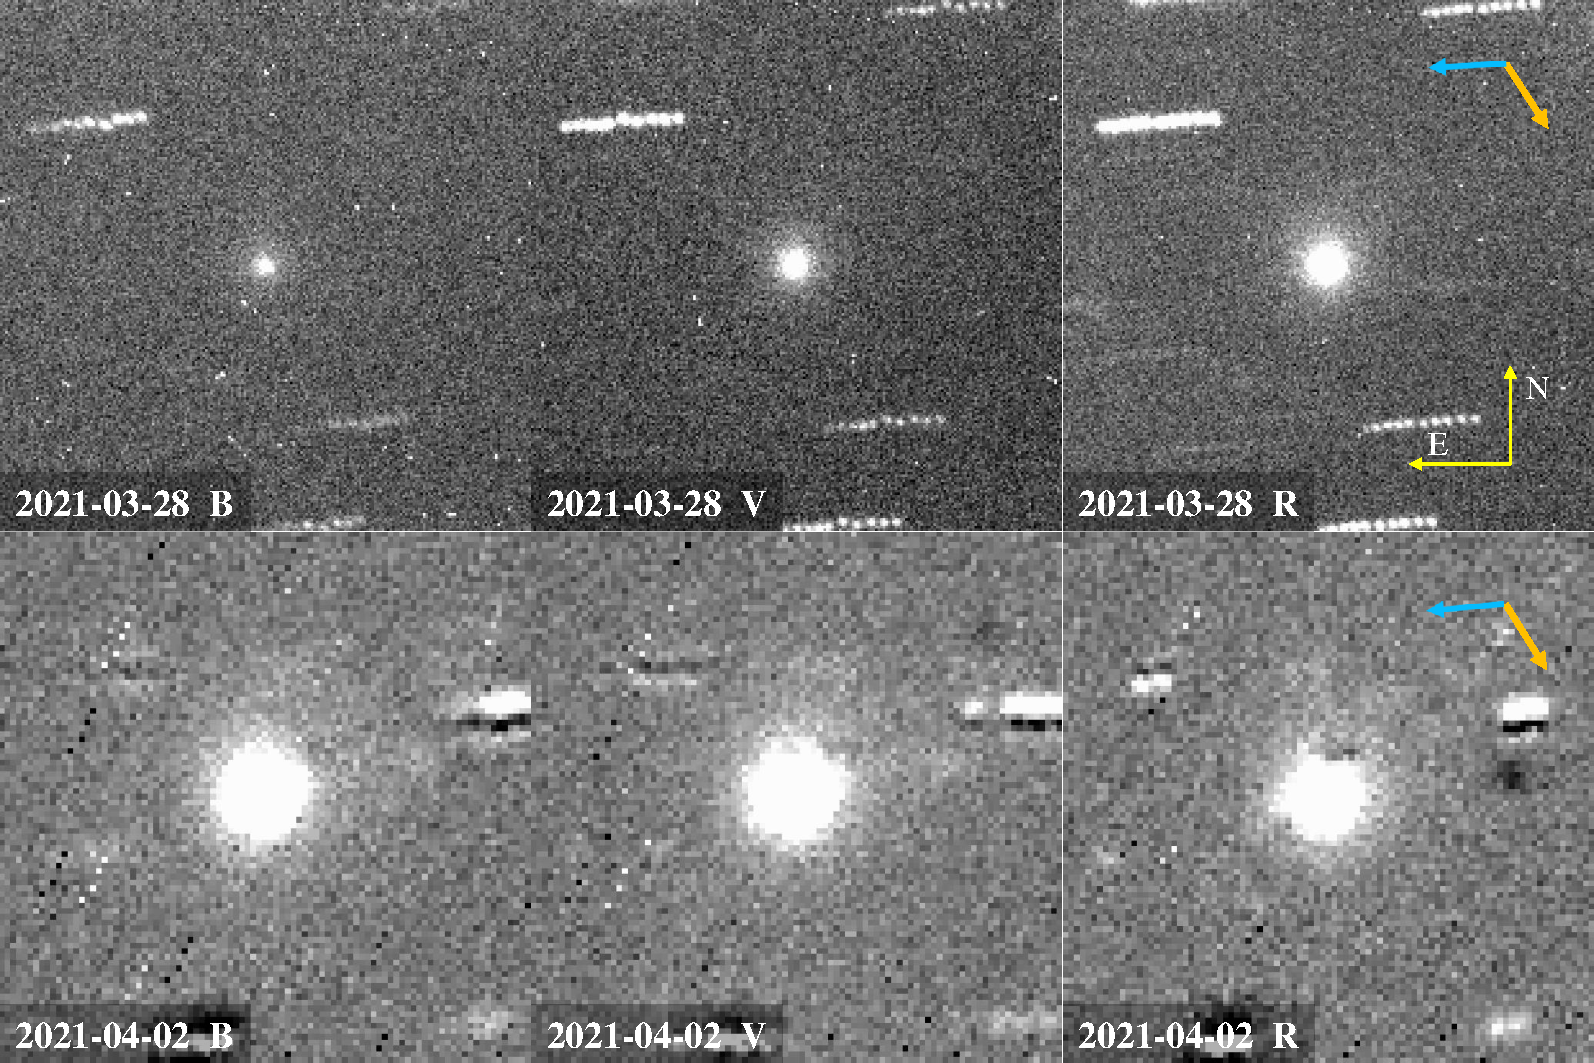
\includegraphics[width=.9\linewidth]{combine1.pdf}
        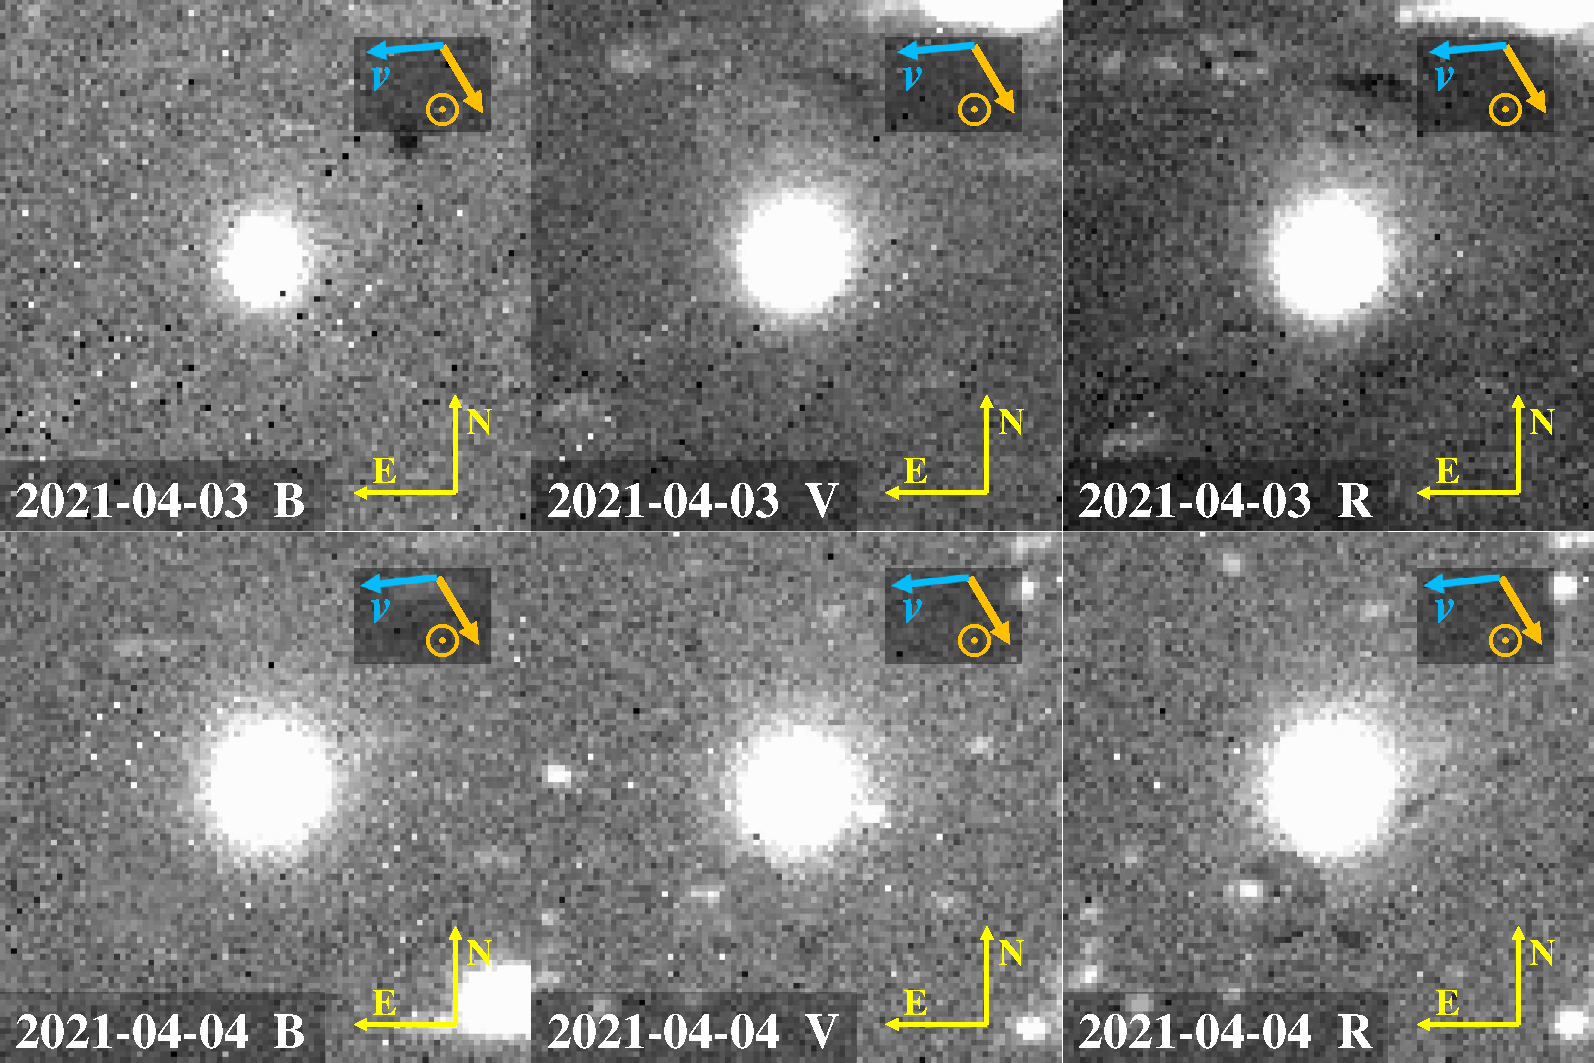
\includegraphics[width=.9\linewidth]{combine2.pdf} 
        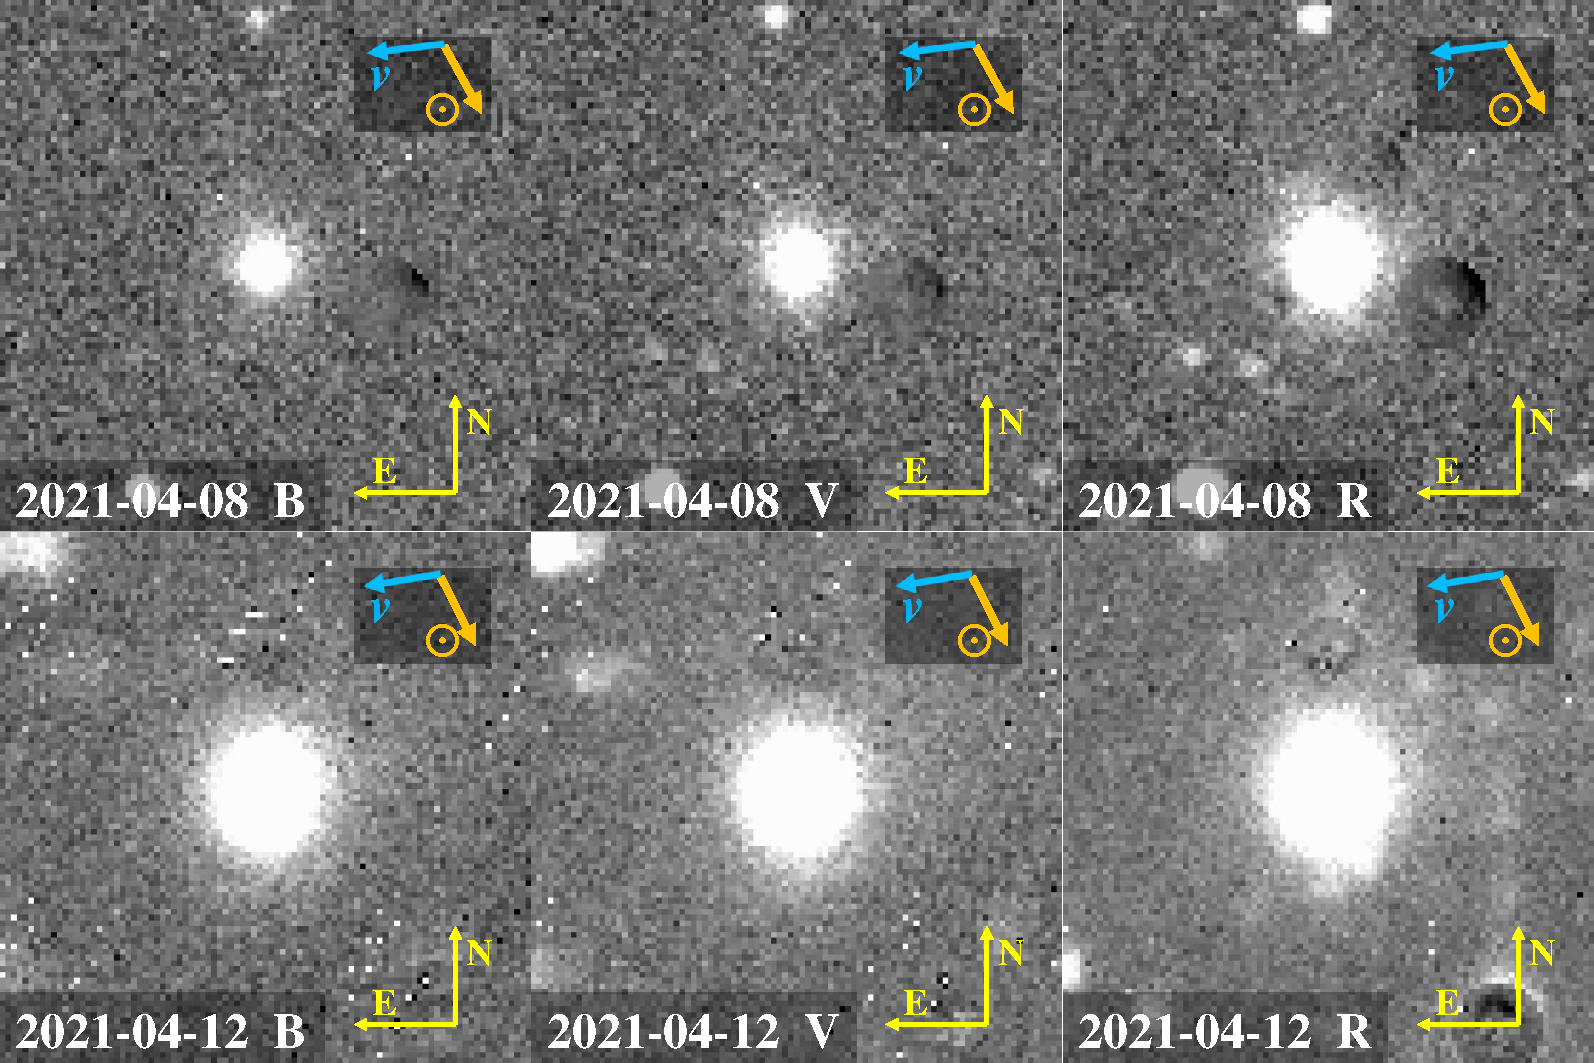
\includegraphics[width=.9\linewidth]{combine3.pdf}
        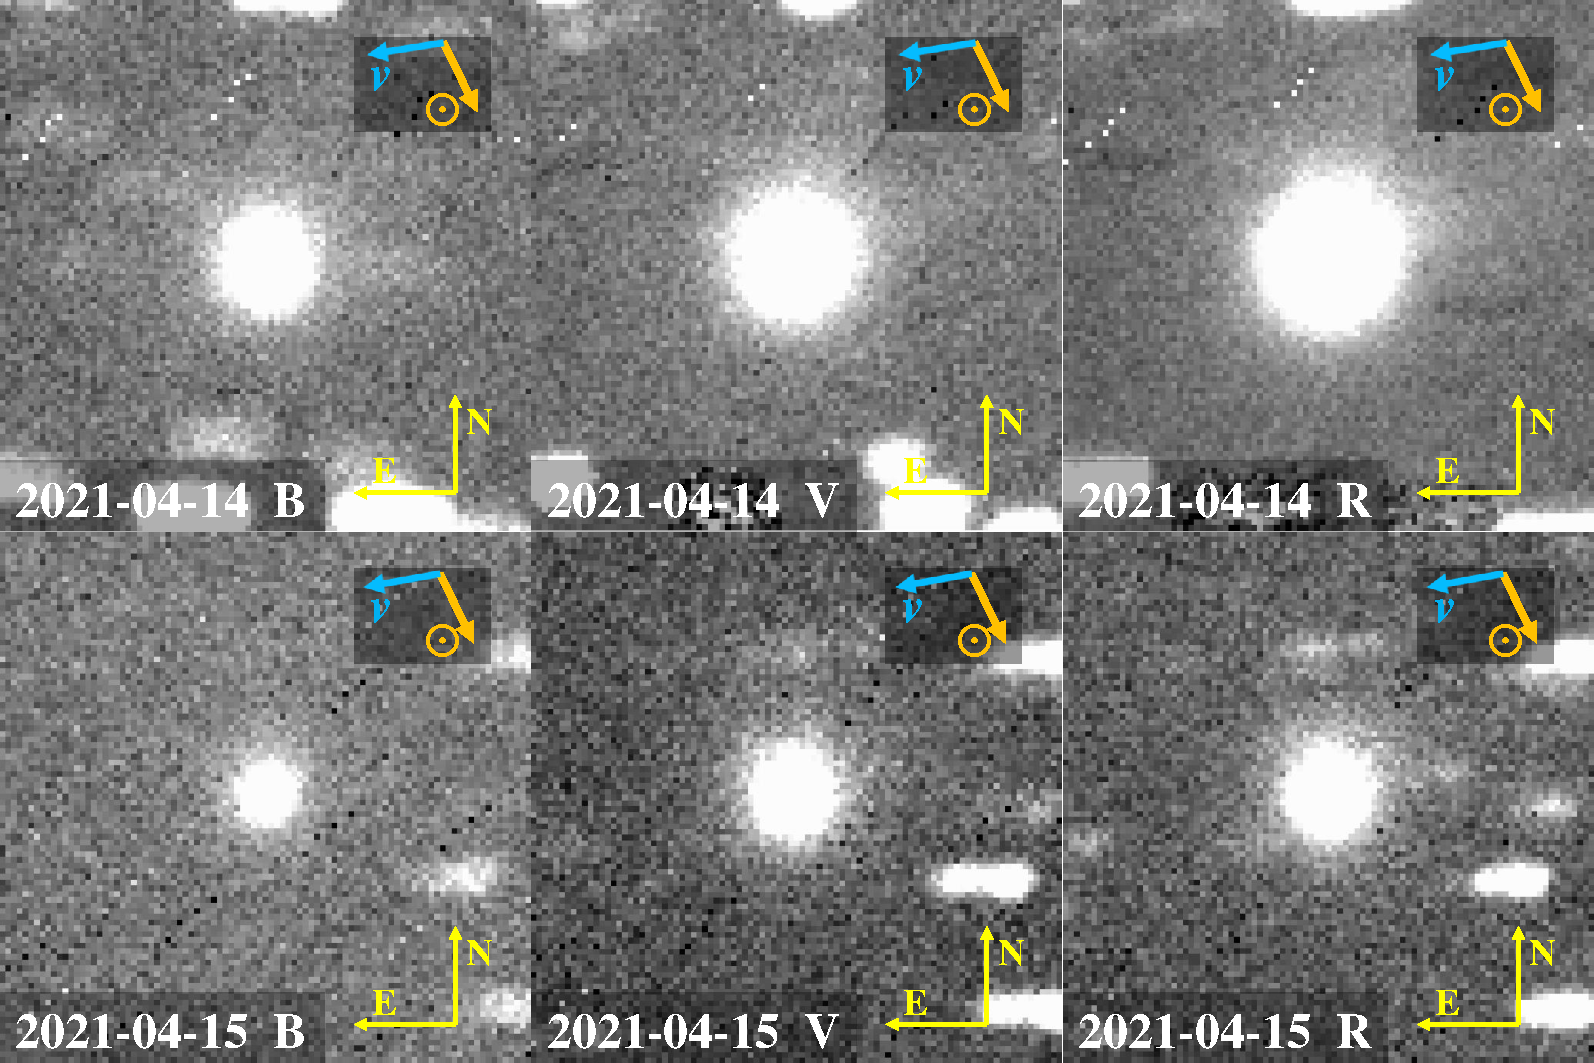
\includegraphics[width=.9\linewidth]{combine4.pdf}
    }
    \caption{The processed images of comet C/2019 L3 and C/2020 P3 in different filters, with north at the top and east to the left. The field of view is $ 2^{\prime} \times 2^{\prime} $ for each thumbnail. Blue arrow shows the direction of the comets' velocity, and the orange arrow shows the direction to the Sun. }
    \label{fig:combinedimg}
\end{figure}

\begin{figure}
    \centering
    \ContinuedFloat
    \subcaptionbox{C/2019 L3}[\linewidth]{
        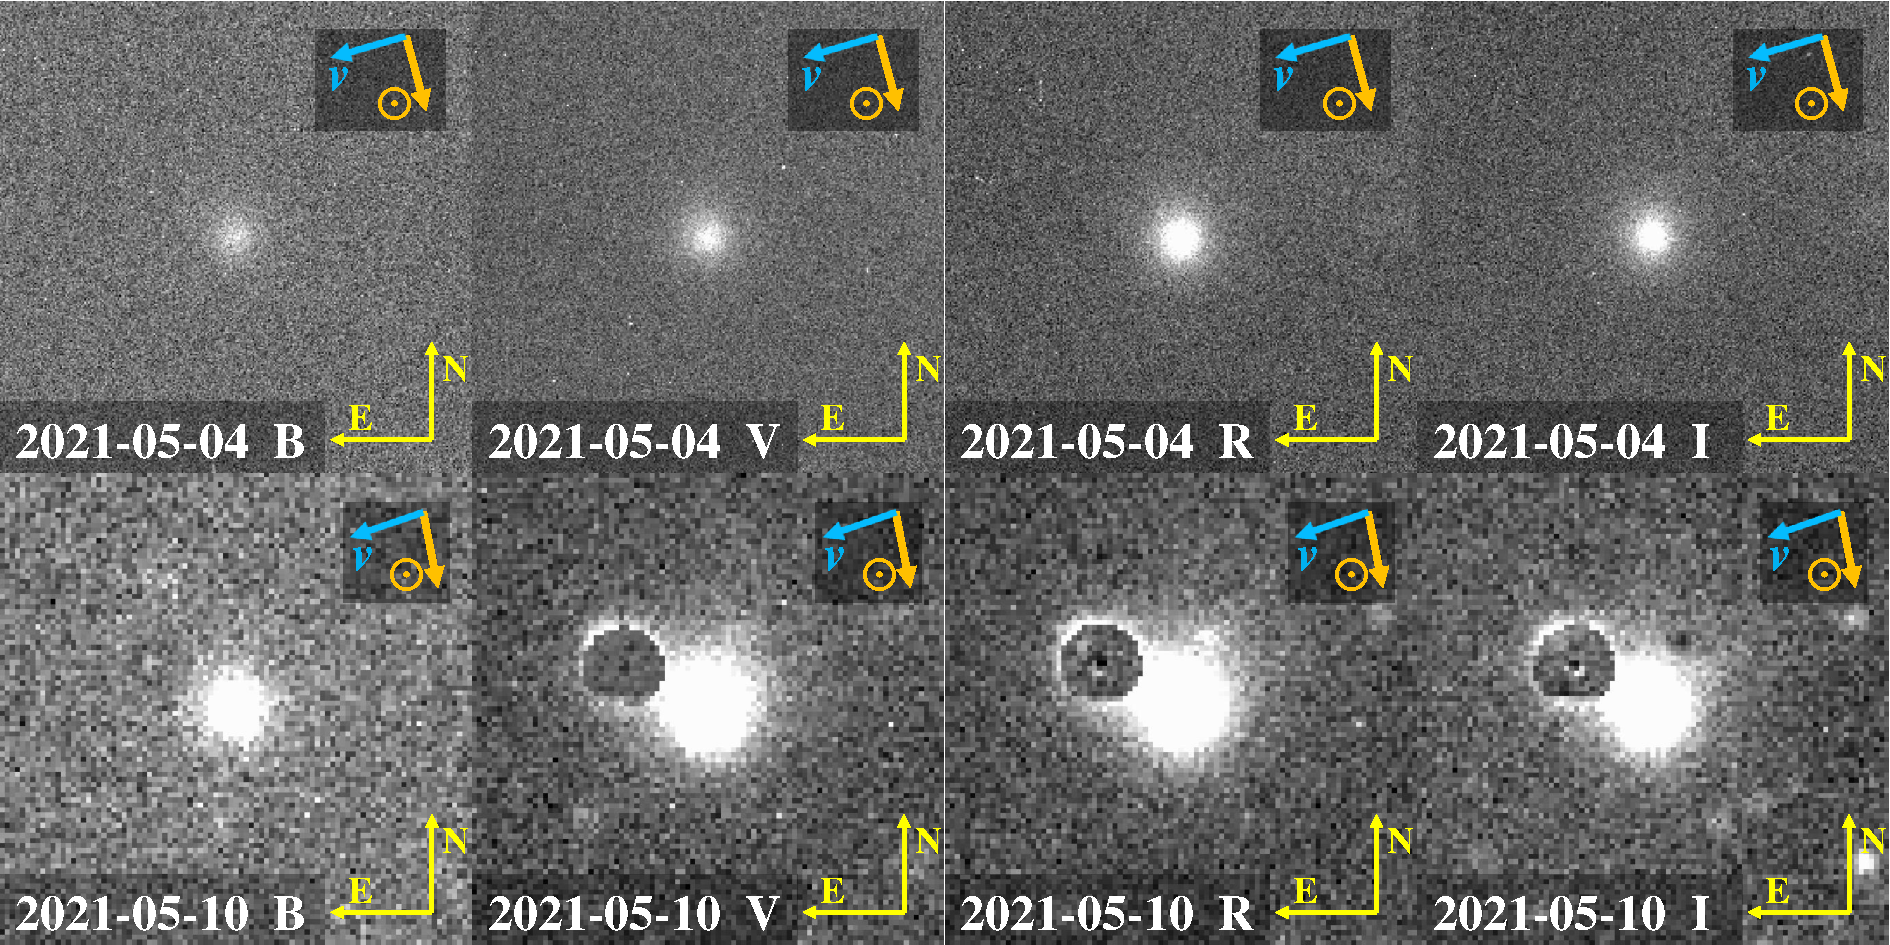
\includegraphics[width=\linewidth]{combine5.pdf}
        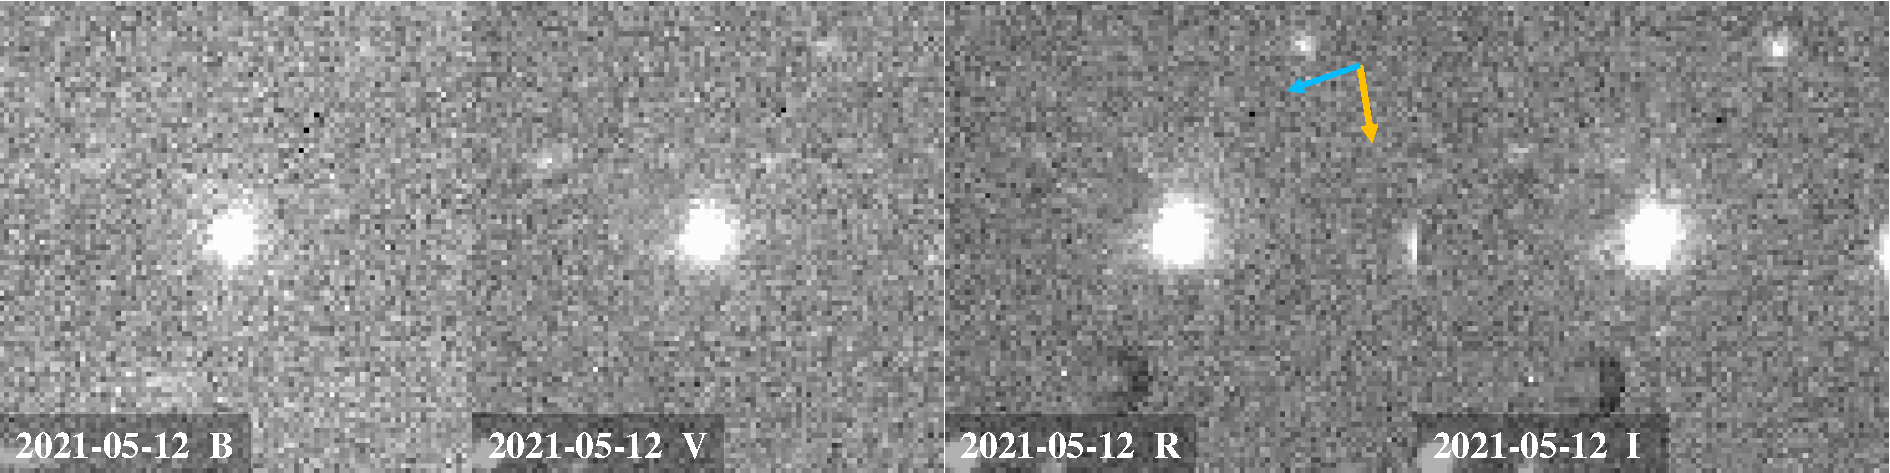
\includegraphics[width=\linewidth]{combine6.pdf} 
        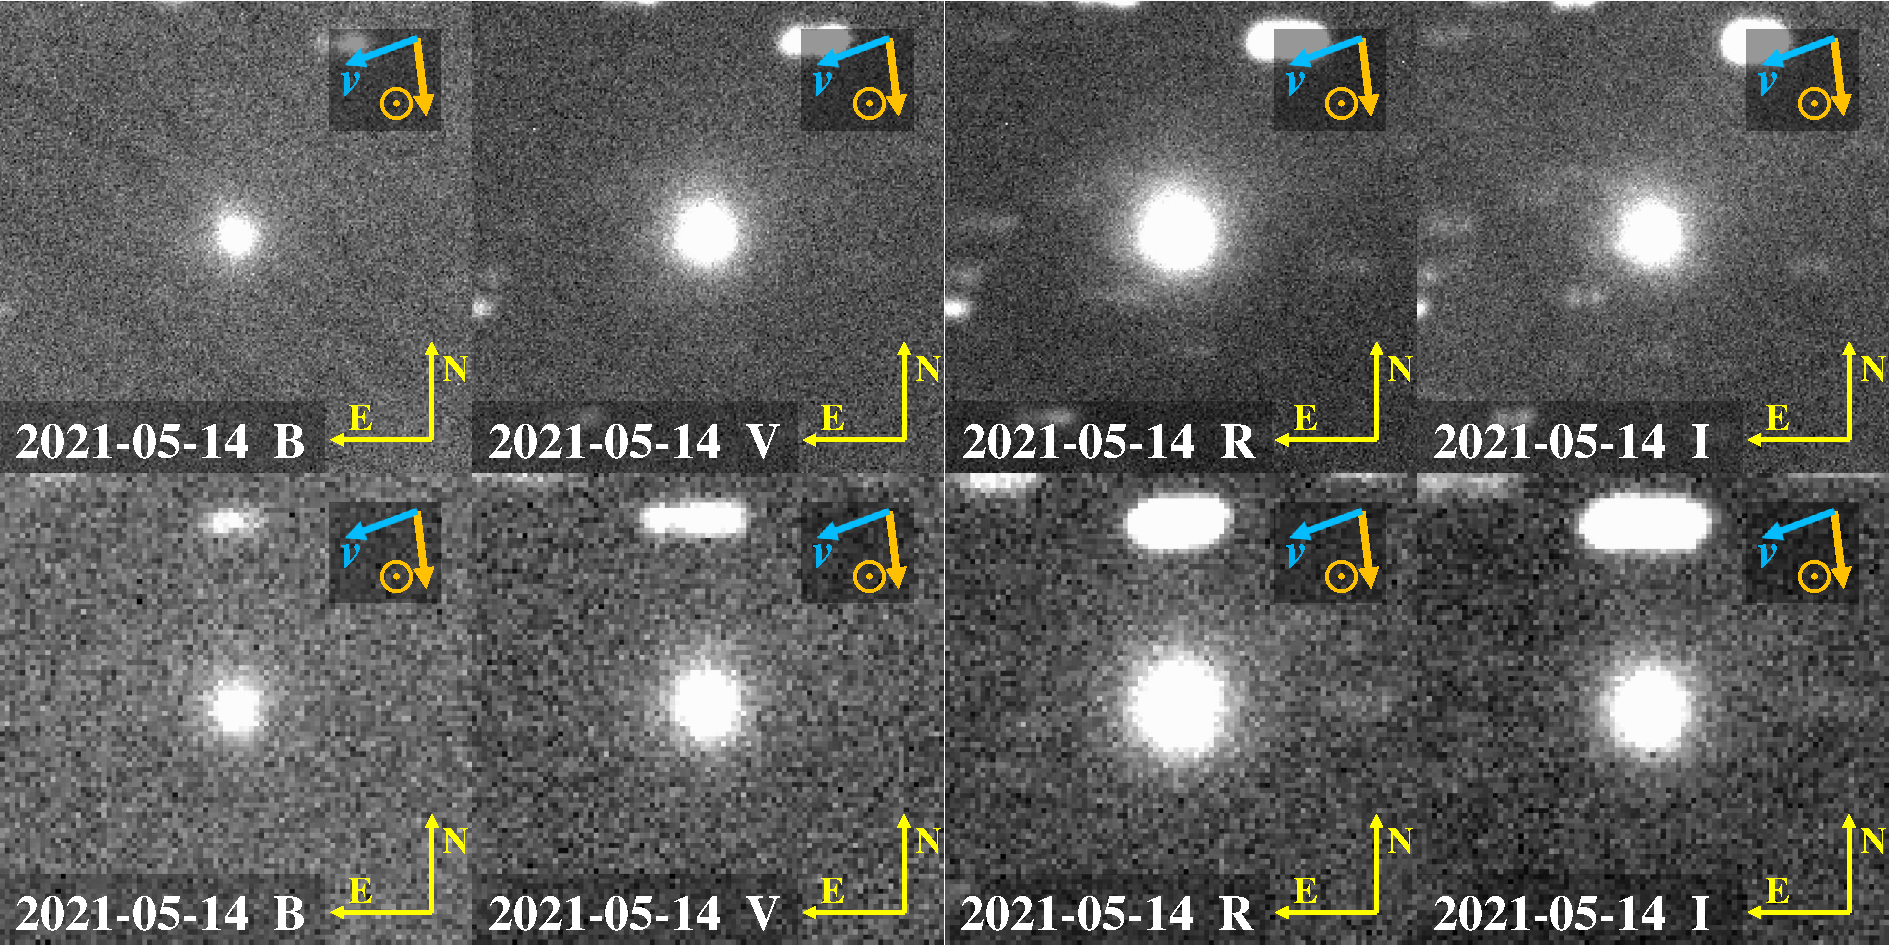
\includegraphics[width=\linewidth]{combine7.pdf} 
    }
        
    \caption{(Continued)}
\end{figure}

\begin{figure}
    \centering
    \ContinuedFloat
    \subcaptionbox{C/2020 P3}[\linewidth]{
        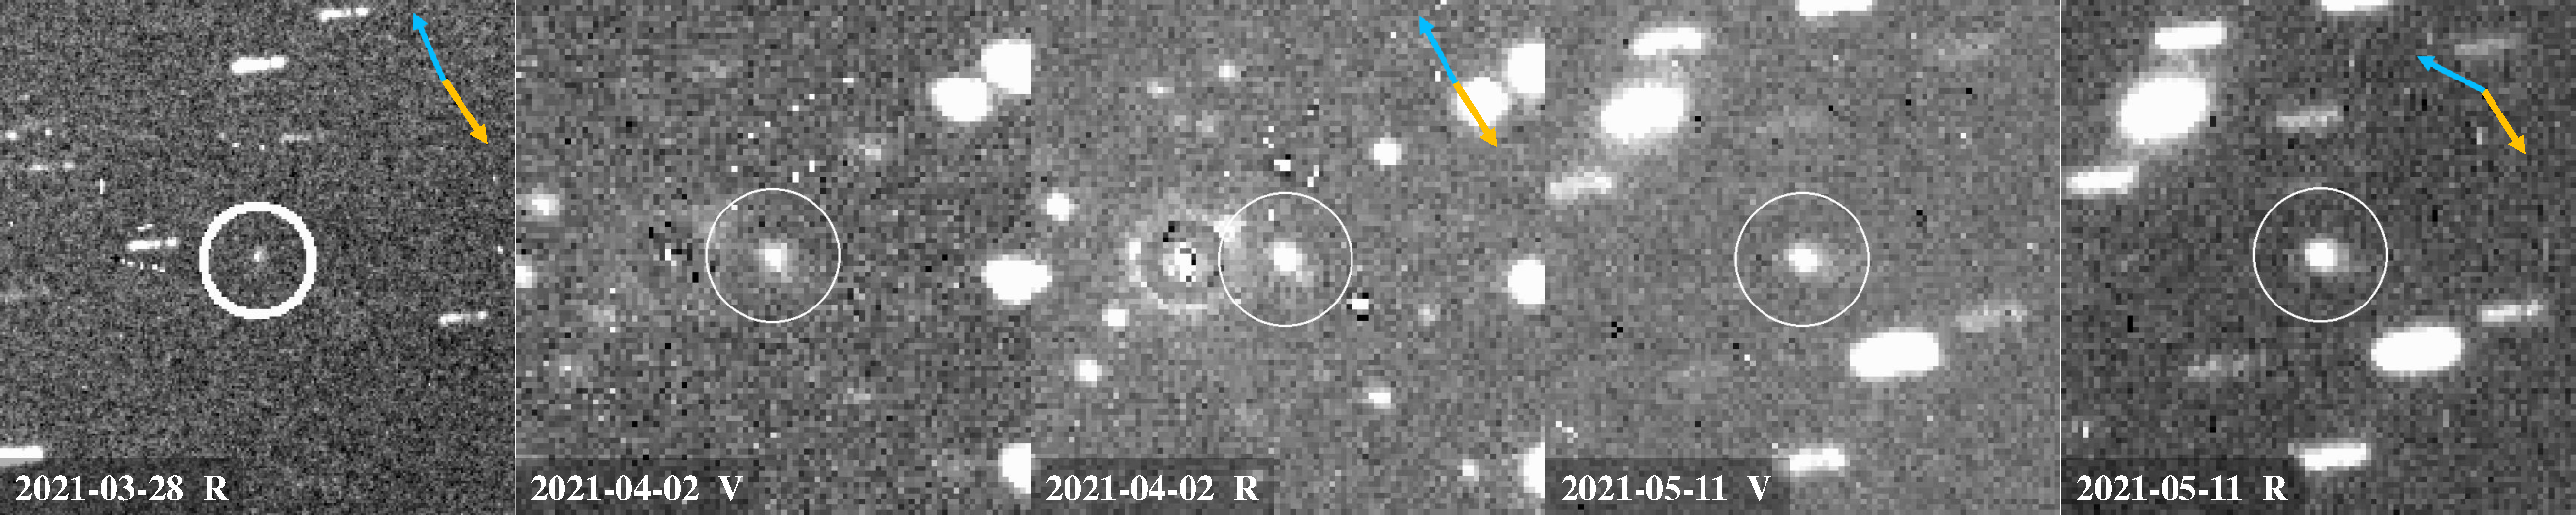
\includegraphics[width=\linewidth]{combine8.pdf}
        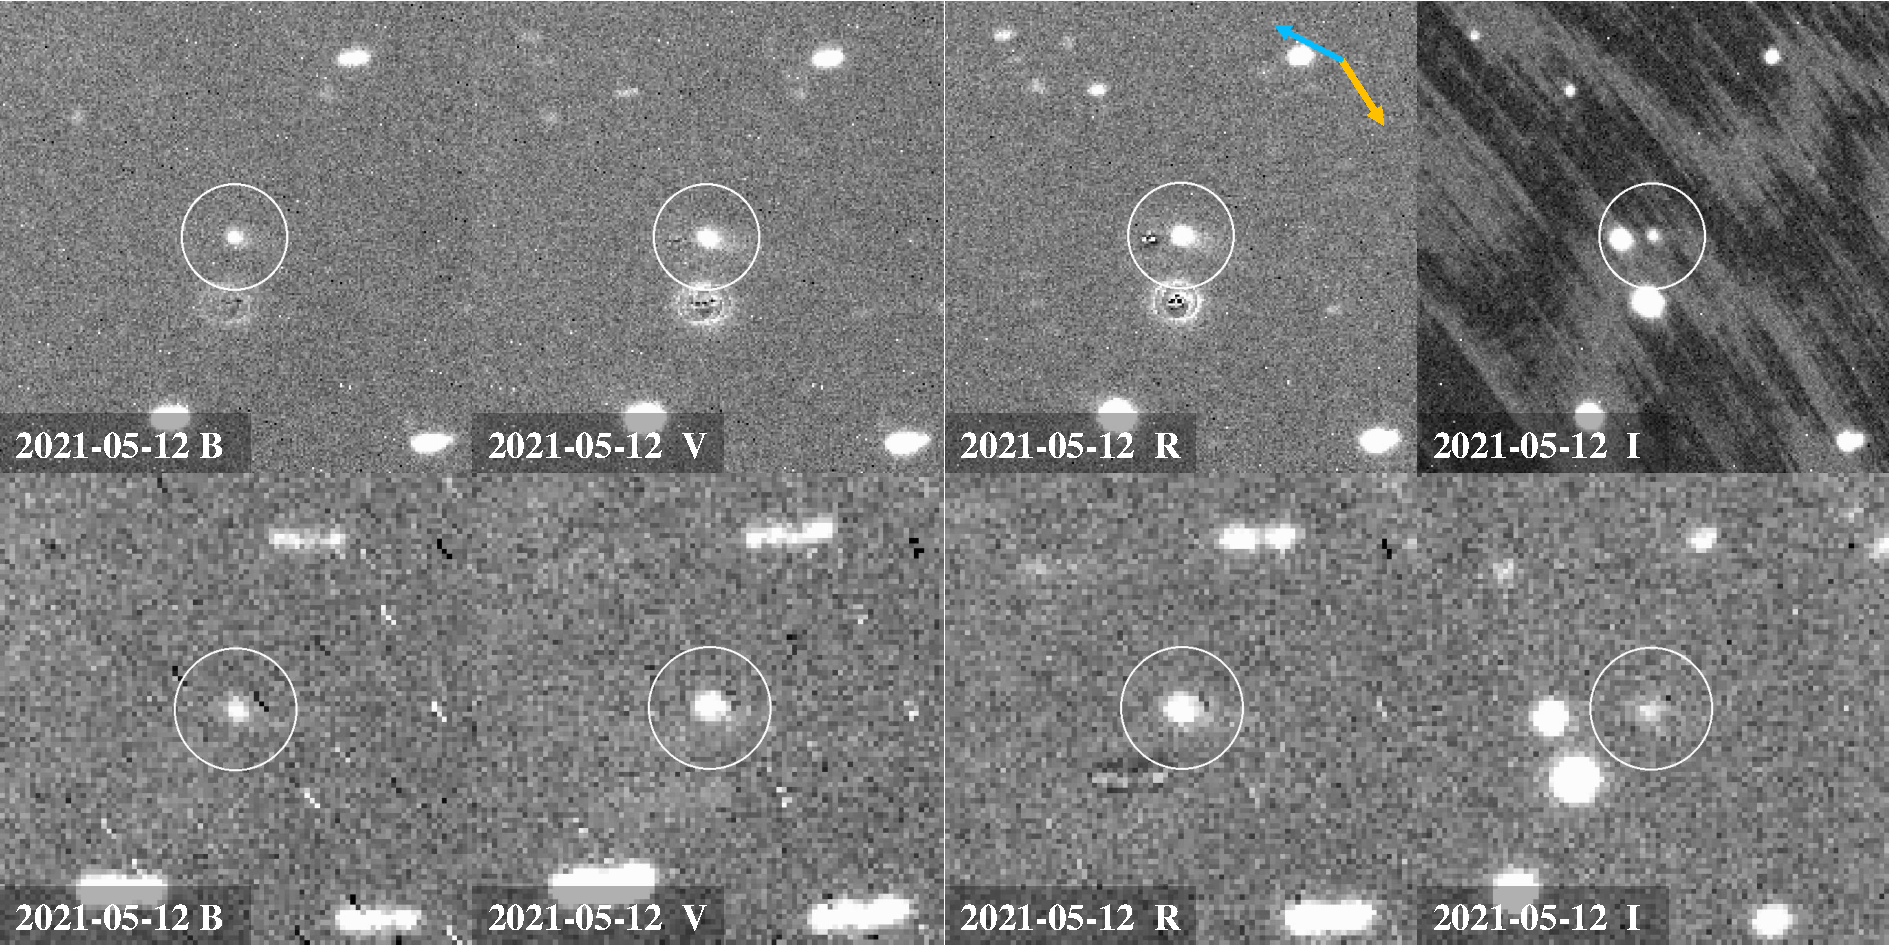
\includegraphics[width=\linewidth]{combine9.pdf} 
    }
    
    \caption{(Continued)}
\end{figure}

\begin{figure}
    \centering
    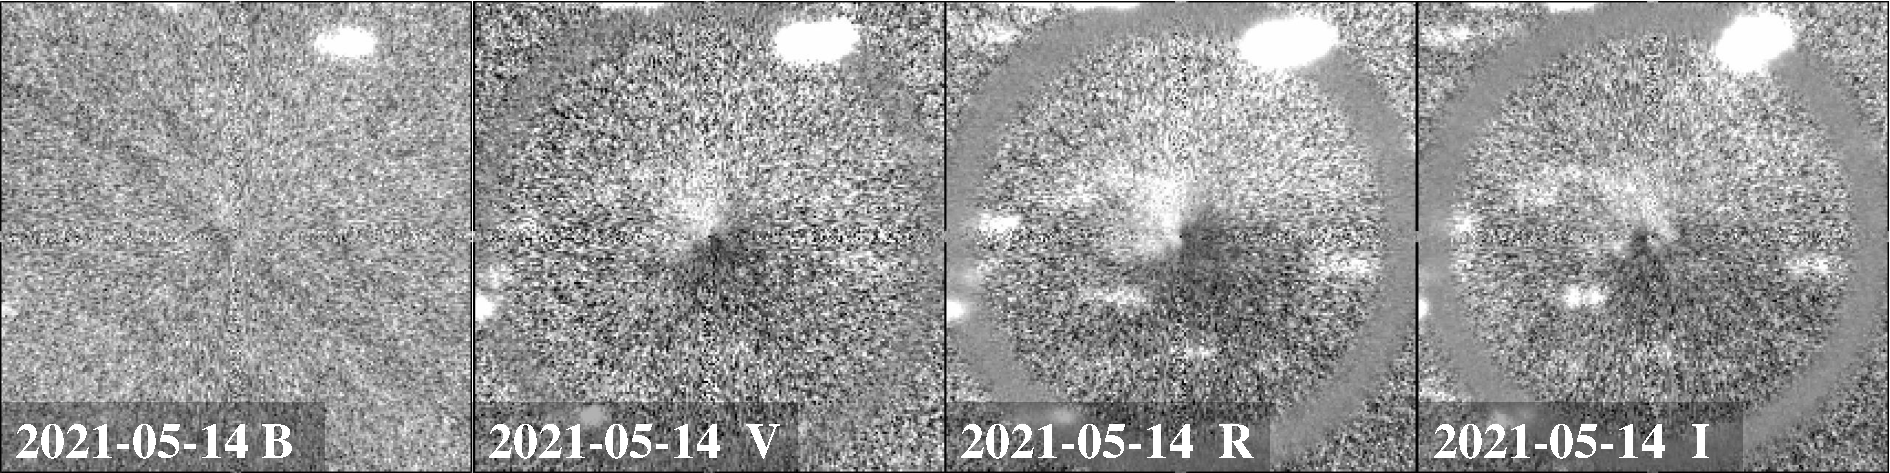
\includegraphics[width=\linewidth]{azi_ren.pdf}
    \caption{Azimuthal renormalized image of C/2019 L3 on \DTMdate{2021-5-14}, the field of view for each thunbnail is also $\ang{;2;}\times\ang{;2;}$. \label{fig:aziren}}
\end{figure}
    
% BVR
\begin{table}
    \centering
    \caption{Photometric results of comet C/2019 L3 and C/2020 P3. }\label{tab:bvr}
    \begin{threeparttable}
        \resizebox{\linewidth}{!}{
        \begin{tabular}{ccccccccc}
            \toprule
            Observation Time\tnote{1} & $\rho\tnote{2}~[^{\prime \prime}]$ & B & V & R & I & $\mathrm{B}-\mathrm{V}$ & $\mathrm{V}-\mathrm{R}$ & $\mathrm{R}-\mathrm{I}$\\
            \midrule
            \multicolumn{9}{l}{\textbf{C/2019 L3}} \\
            2021-03-28.729 & \num{14.5} & \num{14.32 +- 0.09} & \num{13.72 +- 0.07} & \num{13.17 +- 0.15} & - & \num{0.60 +- 0.11} & \num{0.55 +- 0.16} & - \\
            2021-04-02.739 & \num{15.6} & \num{14.37 +- 0.10} & \num{13.62 +- 0.04} & \num{13.14 +- 0.06} & - & \num{0.75 +- 0.11} & \num{0.48 +- 0.07} & - \\
            2021-04-03.719 & \num{15.6} & \num{14.25 +- 0.05} & \num{13.55 +- 0.03} & \num{13.08 +- 0.07} & - & \num{0.70 +- 0.05} & \num{0.47 +- 0.08} & - \\
            2021-04-04.691 & \num{15.6} & \num{14.26 +- 0.05} & \num{13.55 +- 0.02} & \num{13.32 +- 0.01} & - & \num{0.70 +- 0.05} & \num{0.23 +- 0.02} & - \\
            2021-04-08.691 & \num{15.6} & \num{14.33 +- 0.05} & \num{13.44 +- 0.02} & \num{13.36 +- 0.01} & - & \num{0.88 +- 0.05} & \num{0.09 +- 0.03} & - \\
            2021-04-12.724 & \num{19.5} & \num{14.22 +- 0.05} & \num{13.33 +- 0.01} & \num{13.19 +- 0.01} & - & \num{0.89 +- 0.05} & \num{0.14 +- 0.02} & - \\
            2021-04-14.702 & \num{15.6} & \num{14.21 +- 0.04} & \num{13.51 +- 0.03} & \num{13.29 +- 0.02} & - & \num{0.71 +- 0.05} & \num{0.21 +- 0.03} & - \\
            2021-04-15.714 & \num{15.6} & \num{14.23 +- 0.03} & \num{13.51 +- 0.01} & \num{13.28 +- 0.02} & - & \num{0.72 +- 0.04} & \num{0.23 +- 0.02} & - \\
            2021-05-04.736 & \num{11.0} & \num{14.32 +- 0.04} & \num{13.75 +- 0.04} & \num{13.42 +- 0.04} & \num{13.25 +- 0.03} & \num{0.57 +- 0.05} & \num{0.33 +- 0.06} & \num{0.17 +- 0.05} \\
            2021-05-10.735 & \num{15.6} & \num{13.96 +- 0.03} & \num{13.24 +- 0.01} & \num{13.05 +- 0.03} & \num{12.80 +- 0.04} & \num{0.72 +- 0.04} & \num{0.18 +- 0.03} & \num{0.26 +- 0.05} \\
            2021-05-12.724 & \num{15.6} & \num{14.14 +- 0.03} & \num{13.27 +- 0.03} & \num{13.11 +- 0.02} & \num{12.90 +- 0.03} & \num{0.87 +- 0.05} & \num{0.16 +- 0.04} & \num{0.22 +- 0.04} \\
            2021-05-14.721 & \num{14.0} & \num{14.21 +- 0.04} & \num{13.28 +- 0.04} & \num{13.13 +- 0.02} & \num{12.90 +- 0.06} & \num{0.93 +- 0.06} & \num{0.15 +- 0.04} & \num{0.24 +- 0.06} \\
            \multicolumn{9}{l}{\textbf{C/2020 P3}} \\
            2021-04-02.775 & \num{13.0} & - & \num{17.61 +- 0.05} & \num{17.24 +- 0.03} & - & - & \num{0.37 +- 0.05} & - \\
            2021-05-11.744 & \num{13.0} & - & \num{18.15 +- 0.05} & \num{17.83 +- 0.04} & - & - & \num{0.32 +- 0.06} & - \\
            2021-05-12.749 & \num{6.7} & \num{19.00 +- 0.06} & \num{18.05 +- 0.03} & \num{17.88 +- 0.02} & \num{17.67 +- 0.04} & \num{0.95 +- 0.07} & \num{0.17 +- 0.04} & \num{0.21 +- 0.05} \\
            \bottomrule
        \end{tabular}
        }
        \begin{tablenotes}
            \item[1] UT time at the beginning of exposure
            \item[2] the photometric aperture in arcsecond
        \end{tablenotes}
    \end{threeparttable}
\end{table}

\begin{comment}
\subsection{Nucleus size}

For comets observed at large heliocentric distances that are commonly assumed to be inactive, their photometric R magnitude, denoted as $m_R$, can be utilized to derive the maximum estimate for the geometric cross-sectional area of the cometary nucleus. This estimation involves the use of the formula proposed by \cite{lamy_comet_2004} for asteroids observed at high phase angle that can be applied to a spherical body expressed as
\begin{equation}
    A_R a_N^2 < \num{2.24e22} r^2 \Delta^2 10^{0.4\left(m_{\odot} - m_R + \beta \alpha\right)}, 
\end{equation}
where $A_R = 0.04$ is the geometric albedo \citep{lamy_comet_2004}, $a_N$ the radius, $r$ the heliocentric distance in \si{\astronomicalunit}, $\Delta$ the geocentric distance in \si{\astronomicalunit}, $m_{\odot} = -27.15$ the R magnitude of the Sun \citep{willmer_absolute_2018}, $\alpha$ the phase angle, and $\beta = 0.04$ the phase coefficient \citep{lamy_comet_2004}. 
Given that two comets in this work were active during the observational run, we set the photometry aperture equal to stellar FWHM and calculate the background value using a circular region near the comet nucleus to reduce the influence of cometary outbursts, then use differential photometry to get new R magnitude to provide a coarse estimation for the nucleus size. 
The images of comet C/2019 L3 taken on \DTMdate{2021-5-4} and that of C/2020 P3 taken on \DTMdate{2021-5-12} exhibit high resolution and were captured at sufficiently distant heliocentric distance, from which we were able to estimate the upper limits of radii for two comets as follows: C/2019 L3 with a limit of {\SI{75.1 +- 3.5}{\km}}, and C/2020 P3 with a limit of {\SI{26.8 +- 0.7}{\km}}. 

% 在后面讨论一下减除彗发的方法是否可靠 (是否稳态彗发? 稳态时可靠)
\end{comment}

\subsection{Surface brightness profile}

Based on the photometric results, the radial surface brightness profile (SBP) was computed as the function of the angular distance $\rho$ measured from the photocenter of comet. For this purpose, every image was trimmed from the center of the comet, and the sky value was determined by the median of the trimmed image. 
In the case of a steady-state coma, the surface brightness $B$ is expected to follow a power-law relation with $\rho$ as $B \propto \rho^m$, where $-1.5 \leqslant m \leqslant -1.0$, and the index $m$ is often referred to as the gradient ($m=\dif\lg{B} \big/ \dif\lg{\rho}$). As the radiation pressure accelerates the dust particles, the value of $m$ decreases and approaches \si{\num{-1.5}} in the limiting case~\citep{jewitt_surface_1987}. Conversely, if the index $m$ falls below \si{\num{-1.5}}, it suggests the presence of nonsteady dust coma emission \citep{lowry_ccd_1999}.

Not only in single images does comet C/2019 L3 appear like a stellar, but also in stacked images. However, the SBP of C/2019 L3 shows it clearly the excess flux in outer region compared with stellar SBP. In Fig.~\ref{fig:sbp} we report an example plot of the R-band SBP as a function of $\lg{\rho}$ for C/2019 L3 observed on \DTMdate{2021-5-4}. The gradient $m$ in the $0.5 \leqslant \lg{\rho} \leqslant 1.0$ range is calculated by the least-squares fit to $\lg{B}$ versus $\lg{\rho}$. 
In Fig.~\ref{fig:sbp_m}, the gradients of C/2019 L3 on each date are depicted, and the averaged value is indicated by a blue dotted line. 
Note that in Fig.~\ref{fig:sbp} the SBP is expressed as magnitude, and according to the relationship between magnitude and luminous intensity, the slope in such figure should be multiplied by \num{-0.4} to make the gradient $m$. The averaged $m$ is \num{-1.66}, and in most cases it is below \num{-1.5}, indicating that this comet's dust emission is in a nonsteady state. While for comet C/2020 P3, all images taken are so faint and it would bring about a great deal of uncertainty if we calculated its SBP. 

% 考虑放置最大、最小、中位数对应图像
\begin{figure}
    \centering
    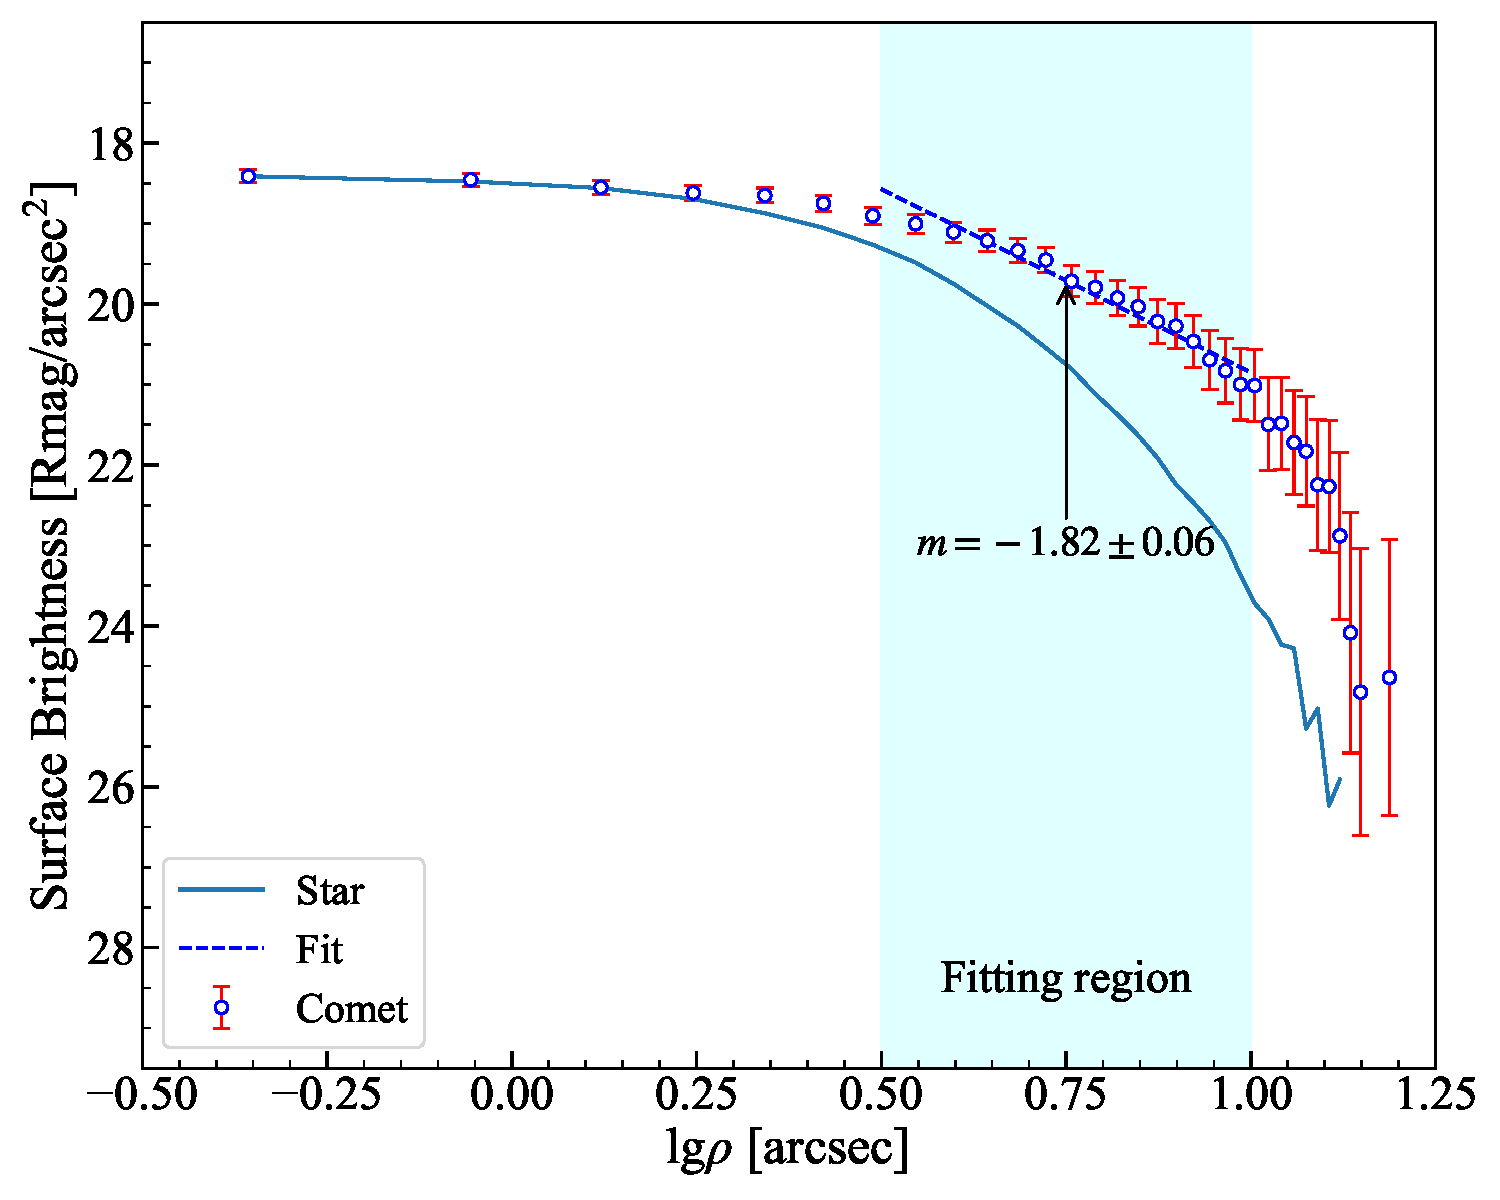
\includegraphics[width=\columnwidth]{sbp-210504-3.pdf}
    \caption{An example figure for R-band surface brightness of comet C/2019 L3. The error plot is the SBP of comet, and the blue solid line is the SBP of a background star. The blue dotted line is a linear regression result of comet's SBP vs $\lg{\rho}$ with $\lg{\rho}$ between 0.5 and 1.0, and the gradient $m$ related to the slope is marked on the graph with an arrow. }
    \label{fig:sbp}
\end{figure}

\begin{figure}
    \centering
    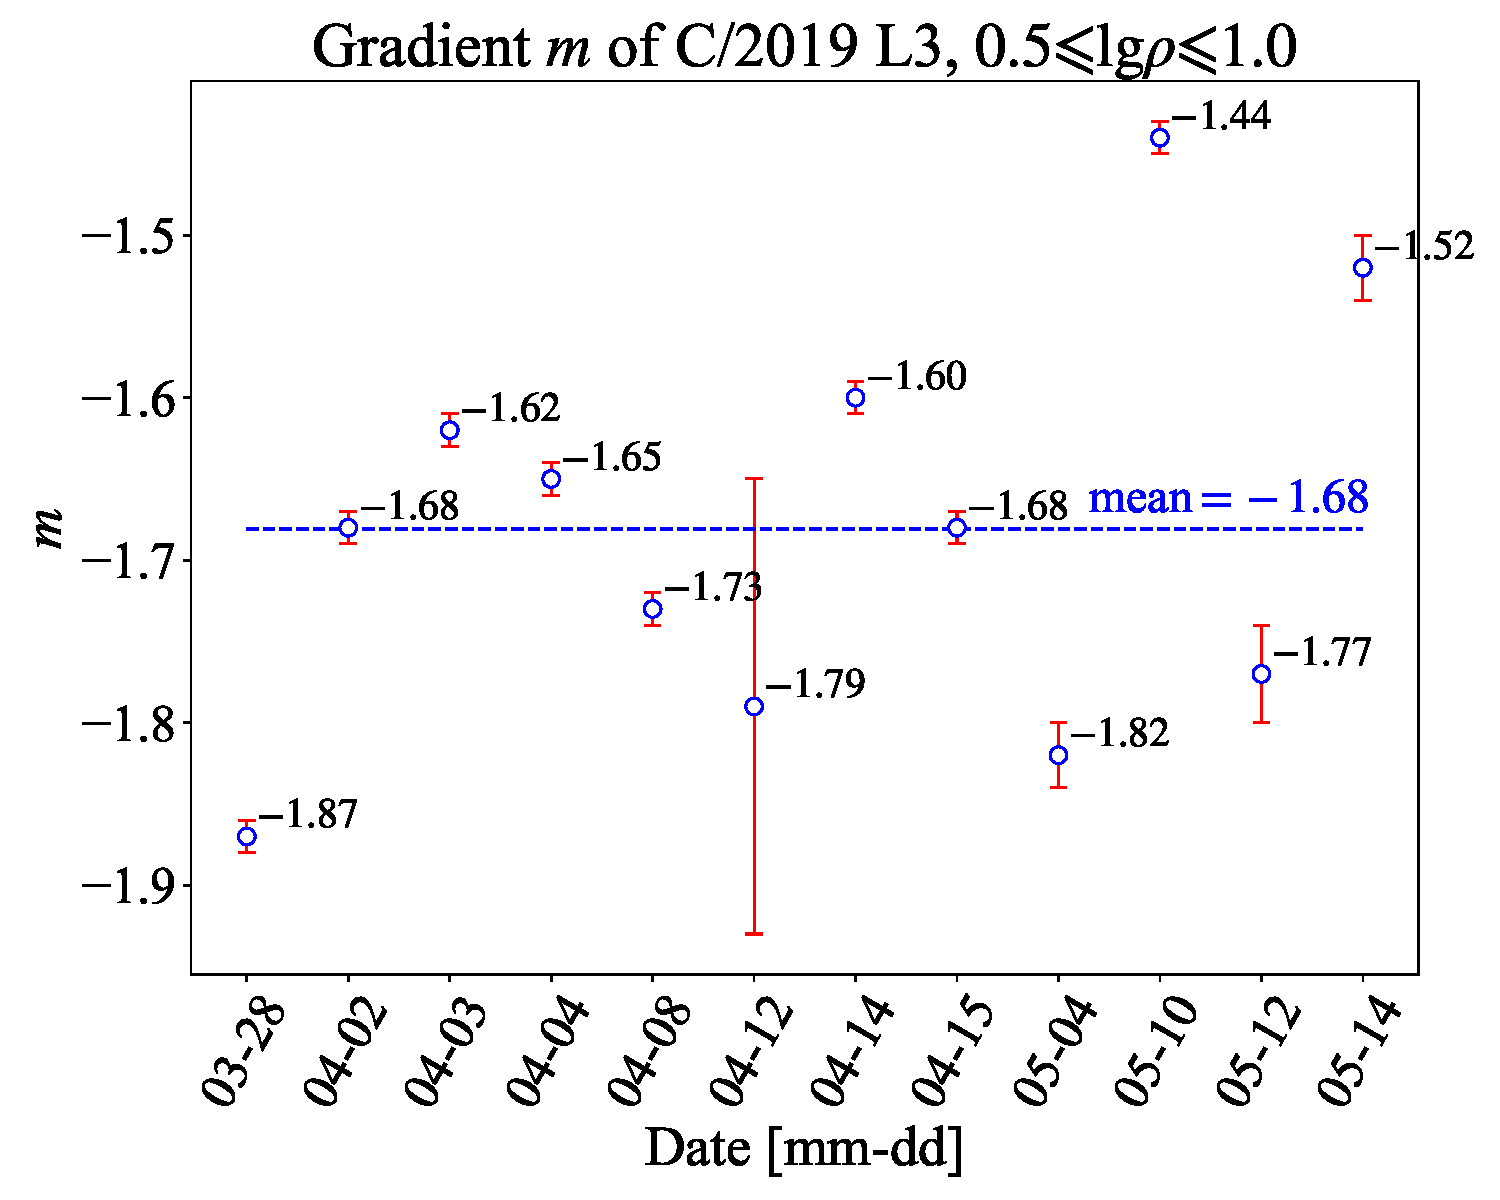
\includegraphics[width=\columnwidth]{sbp_m.pdf}
    \caption{The $m$ of R-band surface brightness of comet C/2019 L3 with date, blue dashed line is the averaged $m$, around which is a red shadow representing the error. }
    \label{fig:sbp_m}
\end{figure}


\subsection{$Af\rho$}

The $Af\rho$ value introduced by \citet{ahearn_comet_1984}, where $A$ represents the grain albedo, $f$ the filling factor, and $\rho$ the aperture, is commonly used to indicate the dust production activity of comets. Usually it is expressed in units of [\unit{\cm}] as equation (\ref{eq:afr}): 
\begin{equation}
    Af\rho = \frac{4 r^2 \Delta^2}{\rho} 10^{0.4(M_\odot - M_\mathrm{c})}, 
    \label{eq:afr}
\end{equation}
where $r$ is the heliocentric distance in units of [\si{\astronomicalunit}], $\Delta$ the geocentric distance in units of [\si{\km}], $\rho$ the aperture in units of [\si{\km}], $M_\odot$ the absolute magnitude of the Sun (respectively \num{-26.13} and \num{-27.15} in B and R bands, see \citealt{willmer_absolute_2018}), and $M_\mathrm{c}$ the corresponding magnitude of comet under the aperture of $\rho$. 

Due to the phase darkening effect, it is necessary to adjust $Af\rho$ values at different phase angles to a specific angle. In this work, all observations were conducted at small phase angles, and we normalize the $Af\rho$ values to a phase angle of \ang{0} using equation (\ref{eq:a0frho}), as shown below:
\begin{equation}
    A(0)f\rho = \frac{A(\alpha)f\rho}{\phi(\alpha)}, \label{eq:a0frho}
\end{equation}
where $\alpha$ is the phase angle, and $\phi$ is the phase function. A composite phase function (see \citealt{schleicher_composition_2011, marcus_forward-scattering_2007}) suggested by D. Schleicher\footnote{\url{https://asteroid.lowell.edu/comet/dustphase.html}} is suitable for adjustion in this work. The related tabular data (\verb|dustphaseHM_table.txt|\footnote{\url{https://asteroid.lowell.edu/comet/dustphaseHM_table.html}}) provides the phase function with phase angle in the $\ang{0} \leqslant \alpha \leqslant \ang{180}$ range, and we adopt cubic spline interpolation method on it to obtain unlisted values. 

Fig.~\ref{fig:Afrho} shows some part of the R-band $Af\rho$ profiles, and results for the maximum of $Af\rho$ as well as the corresponding aperture on each date are summarised in Table~\ref{tab:afrho}. When a comet possesses steady coma, its $Af\rho$ will be independent of aperture. In this paper, as is shown in Fig.~\ref{fig:Afrho}, that is not the case for comet C/2019 L3 or C/2020 P3, both of which reveal a steep increse in $Af\rho$ with the aperture $\rho$ near the comet center along with a smooth decrese with larger aperture. The increase results from usually the effect of seeing and observational circumstance, while the nonsteady dust emmission and possibly the fading or destruction of dust grain bring the decrease \citep{lara_behaviour_2003,tozzi_imaging_2003}.  
             
% 可选择相同日心距范围内的其他长周期彗星进行比较

%其中,$r$表示日心距(以AU为单位),$\Delta$表示地心距(以km为单位),$\rho$表示以km为单位的孔径,$M_\odot$和$M_c$分别表示太阳和彗星的星等。在比较不同彗星的活动性时,通常以$\rho = 10^4km$为基准比较它们$Af\rho$值的大小。

\begin{figure}
    \centering
    % \subcaptionbox{}{
    %     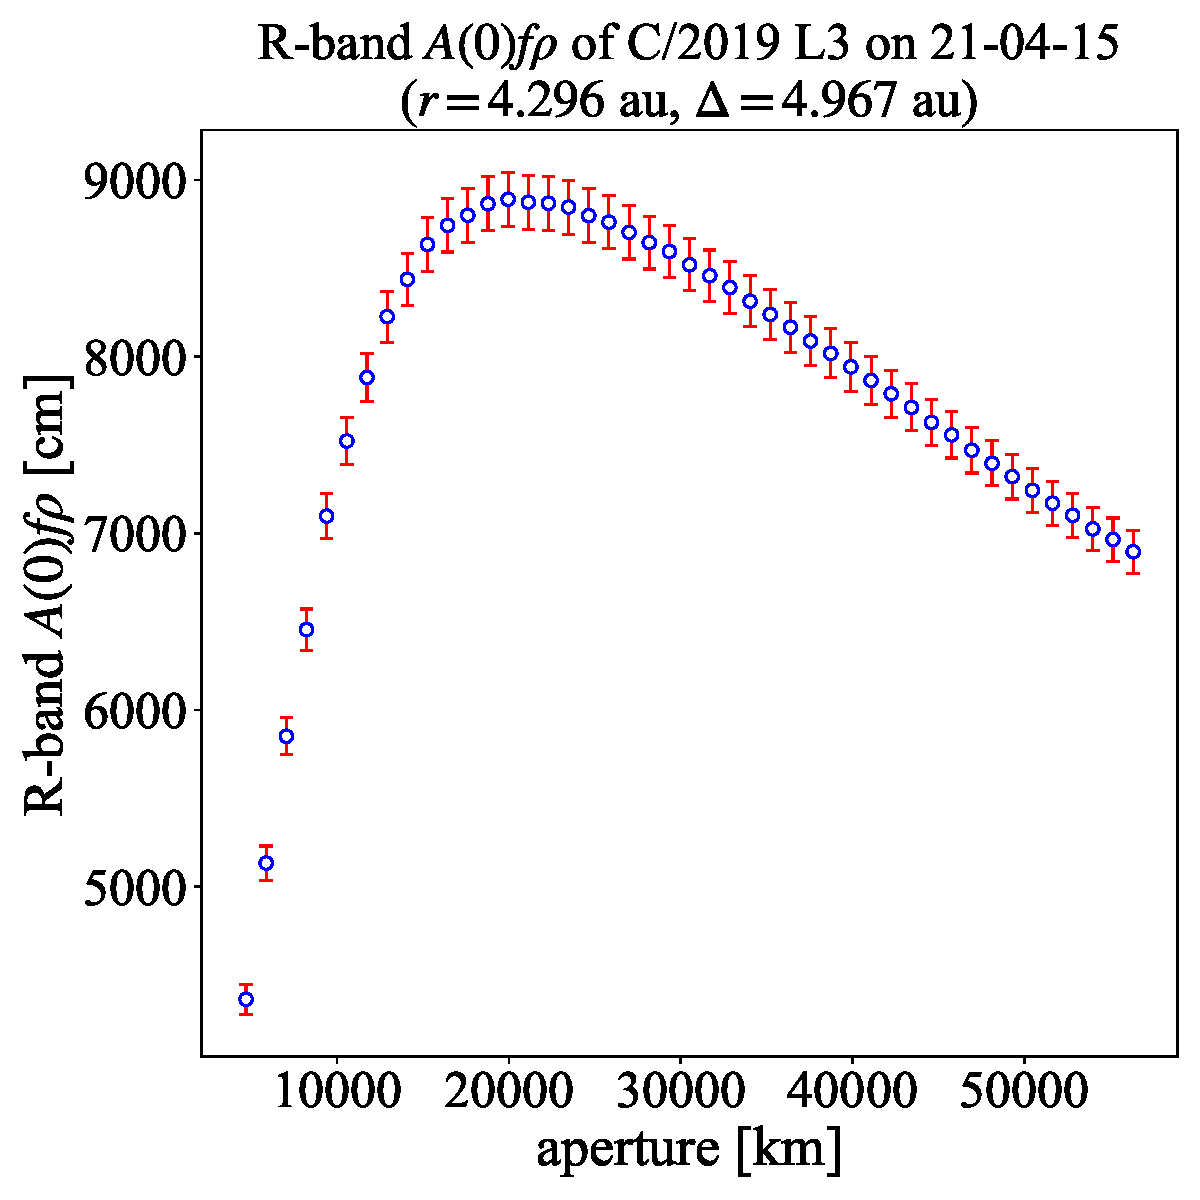
\includegraphics[width=.6\columnwidth]{R-Afrho-C2019L3-210415.pdf}
    % }
    \subcaptionbox{R-band $A(0)f\rho$ of comet C/2019 L3 on \DTMdate{2021-5-14}}{
        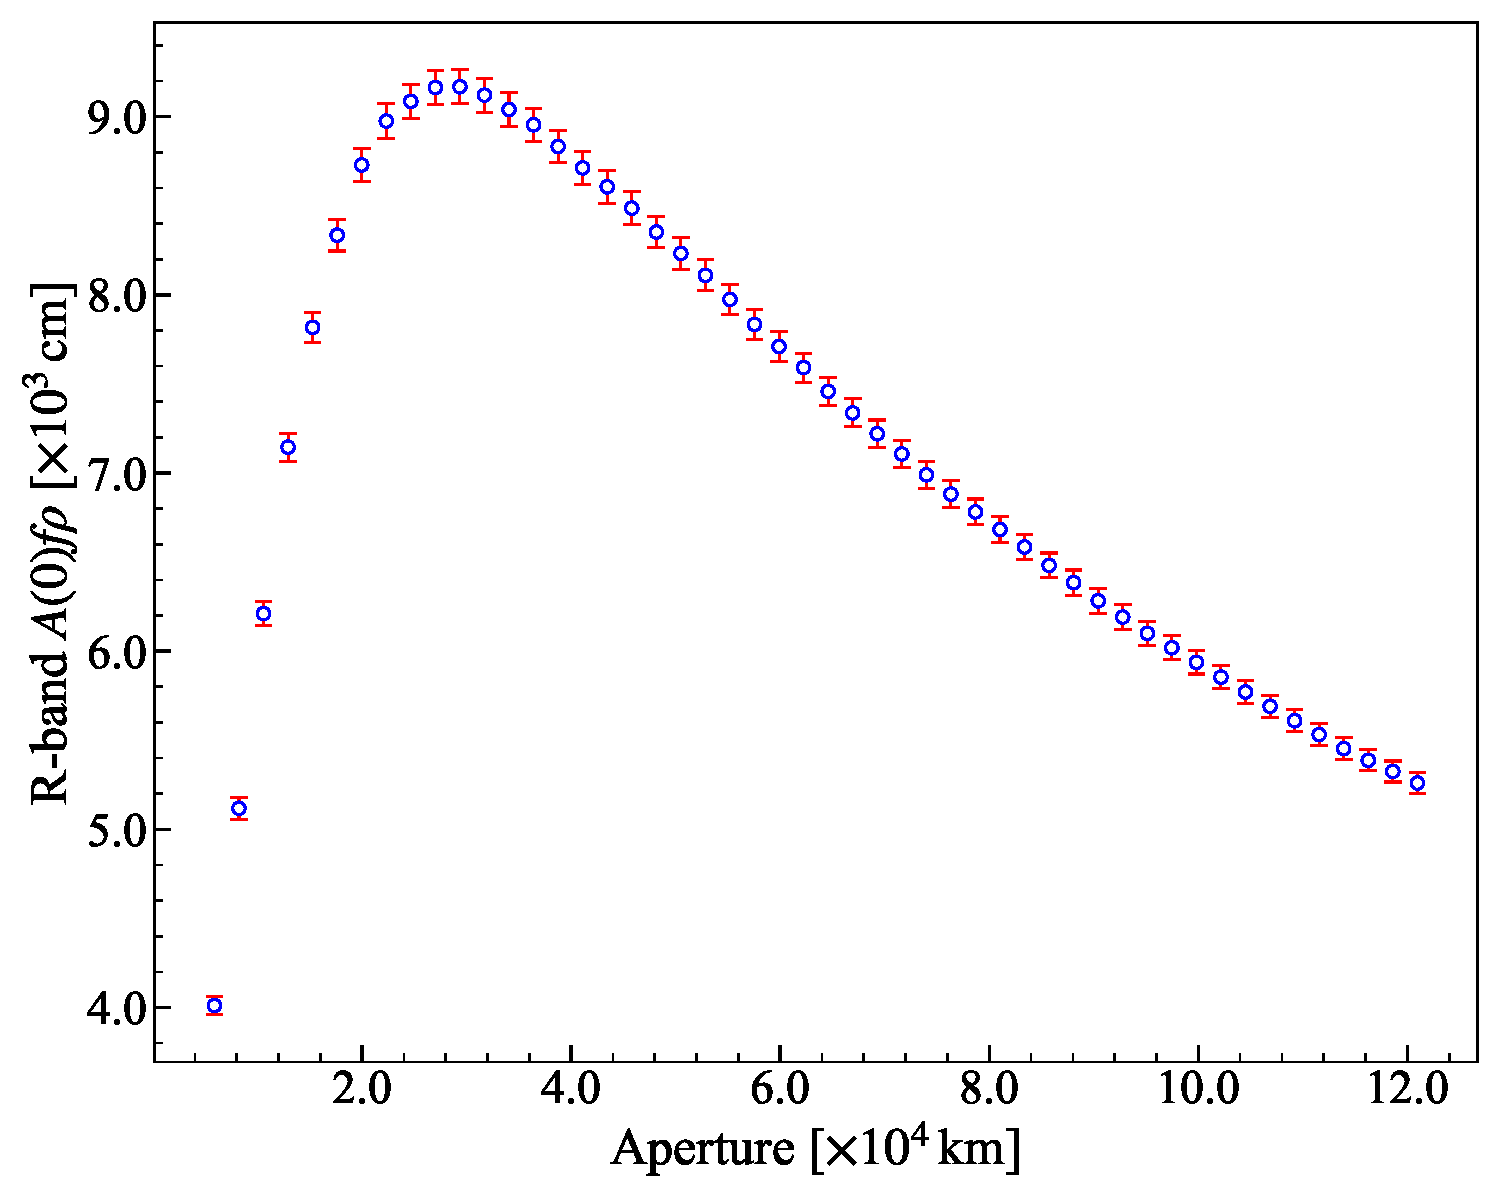
\includegraphics[width=.98\columnwidth]{R-A0frho-C2019L3-210514-119.pdf}
    }

    \subcaptionbox{R-band $A(0)f\rho$ of comet C/2020 P3 on \DTMdate{2021-4-2}}{
        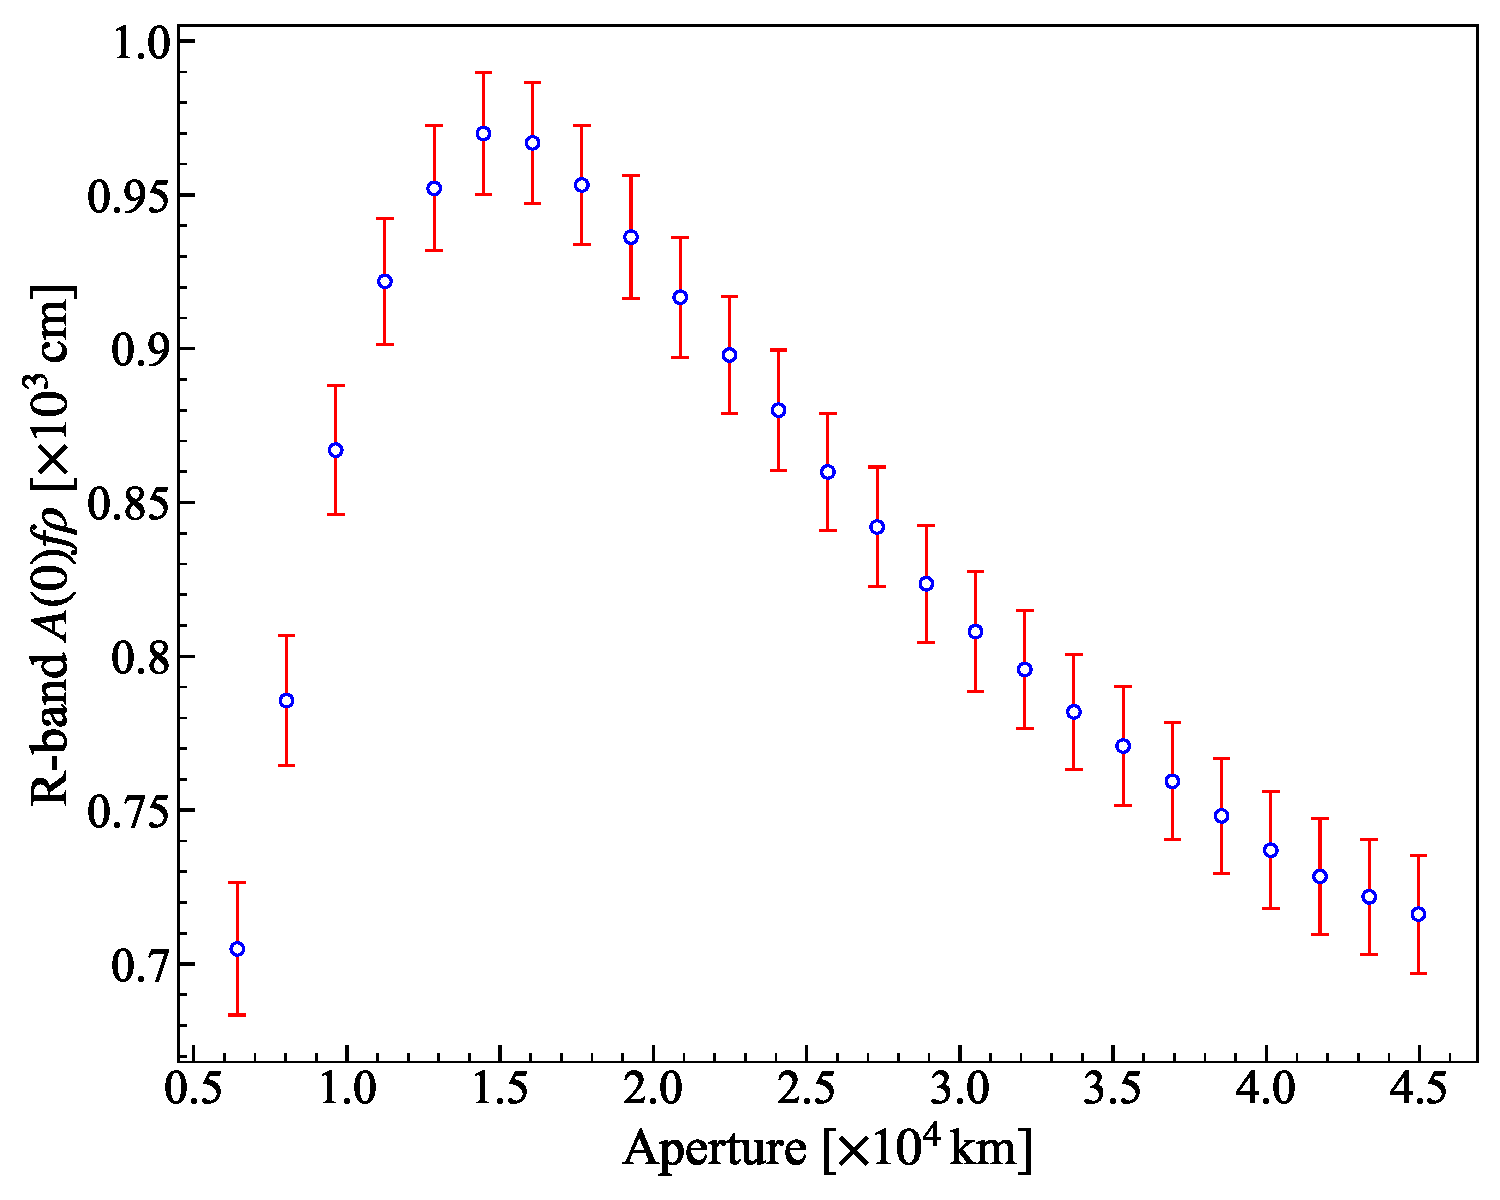
\includegraphics[width=.98\columnwidth]{R-A0frho-C2020P3-210402.pdf}
    }
    % \subcaptionbox{}{
    %     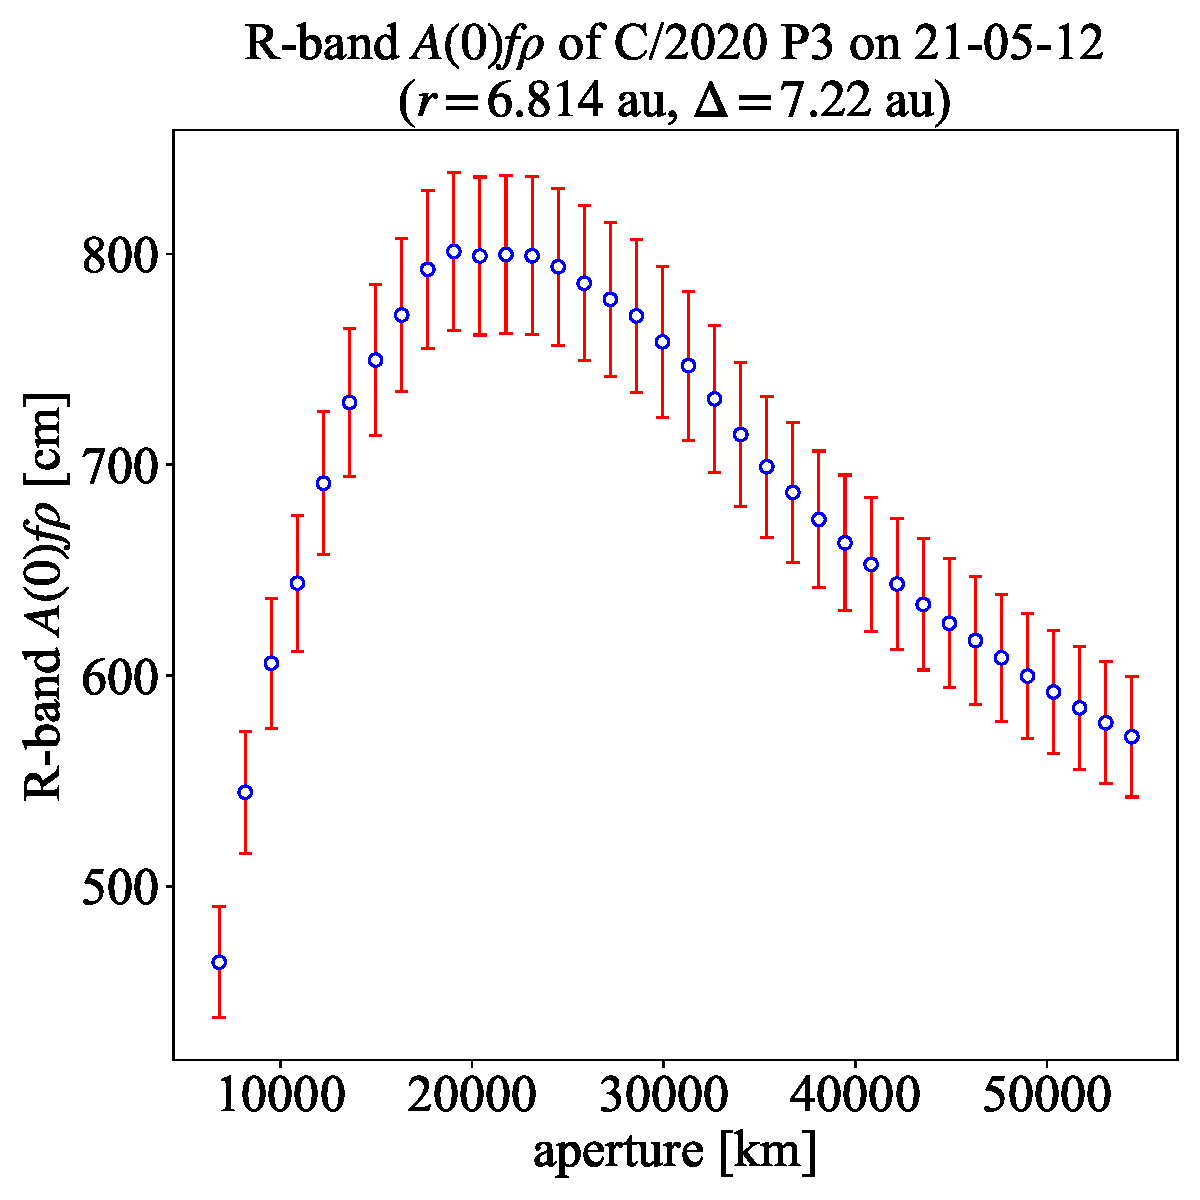
\includegraphics[width=.6\columnwidth]{R-Afrho-C2020P3-210512.pdf}
    % }
    \caption{R-band $A(0)f\rho$ of comet C/2019 L3 and C/2020 P3. }
    \label{fig:Afrho}
\end{figure}

% 统一至20000km?
% Afrho
\begin{table}
    \centering
    \caption{$Af\rho$ values for comet C/2019 L3 and C/2020 P3. }\label{tab:afrho}
    \begin{threeparttable}
        \resizebox{\linewidth}{!}{
        \begin{tabular}{cccc}
            \toprule
            Observation Time & \makecell{$Af\rho$ [\si{\cm}] \\ ($\rho =$ \SI{e4}{\km})} & $Af\rho_\mathrm{max}$ [\si{\cm}] & $\rho_\mathrm{max}$ [\si{\km}]\\
            \midrule
            \multicolumn{4}{l}{\textbf{C/2019 L3}} \\
            2021-03-28.729 & \num{13611 +- 1874} & \num{13615 +- 1875} & \num{10373} \\
            2021-04-02.739 & \num{9332 +- 539} & \num{10748 +- 618} & \num{20930} \\
            2021-04-03.719 & \num{7959 +- 143} & \num{10869 +- 729} & \num{22093} \\
            2021-04-04.691 & \num{6220 +- 69} & \num{9003 +- 114} & \num{20930} \\
            2021-04-08.691 & \num{8985 +- 603} & \num{8700 +- 110} & \num{19860} \\
            2021-04-12.724 & \num{7911 +- 102} & \num{7410 +- 269} & \num{29343} \\
            2021-04-14.702 & \num{7320 +- 95} & \num{8268 +- 133} & \num{25822} \\
            2021-04-15.714 & \num{5043 +- 244} & \num{8891 +- 154} & \num{19953} \\
            2021-05-04.736 & \num{5943 +- 96} & \num{8320 +- 340} & \num{29365} \\
            2021-05-10.735 & \num{7523 +- 134} & \num{8787 +- 205} & \num{29343} \\
            2021-05-12.724 & \num{5701 +- 236} & \num{9590 +- 157} & \num{21127} \\
            2021-05-14.721 & \num{6356 +- 152} & \num{9164 +- 95} & \num{29343} \\
            \multicolumn{4}{l}{\textbf{C/2020 P3}} \\
            2021-04-02.775 & \num{869 +- 20} & \num{948 +- 19} & \num{15789} \\
            2021-05-11.744 & \num{708 +- 17} & \num{848 +- 17} & \num{19048} \\
            2021-05-12.749 & \num{606 +- 31} & \num{801 +- 38} & \num{19048} \\
            \bottomrule
        \end{tabular}
        }
    \end{threeparttable}
\end{table}


\begin{comment}
\begin{figure}[h]
    %\centering
    %\begin{subfigure}{0.5\textwidth}
    \ContinuedFloat
        \subcaptionbox{}{
            \includegraphics[width=.48\linewidth]{Afrho_C2019_4.pdf}
        }
        \subcaptionbox{}{
            \includegraphics[width=.48\linewidth]{Afrho_C2019_5.pdf}
        }

        \subcaptionbox{}{
            \includegraphics[width=.48\linewidth]{Afrho_C2019_6.pdf}
        }
        \subcaptionbox{}{
            \includegraphics[width=.48\linewidth]{Afrho_C2019_7.pdf}
        }
    %\label{fig:first}
    %\end{subfigure}
    \caption{(续)$Af\rho$ of comet C/2019 L3 and C/2020 P3.}
\end{figure}
\end{comment}

\begin{comment}
\begin{figure}[h]
    %\centering
    %\begin{subfigure}{0.5\textwidth}
    
        \subcaptionbox{}{
            \includegraphics[width=.48\linewidth]{Afrho_C2019_0.pdf}
        }
        \subcaptionbox{}{
            \includegraphics[width=.48\linewidth]{Afrho_C2019_1.pdf}
        }

    %\label{fig:first}
    %\end{subfigure}
    \caption{$Af\rho$ of comet C/2019 L3 and C/2020 P3.}
    \label{fig:Afrhomax}
\end{figure}
\begin{figure}[h]
    \ContinuedFloat
    %\centering
    %\begin{subfigure}{0.5\textwidth}
    
        \subcaptionbox{}{
            \includegraphics[width=.48\linewidth]{Afrho_C2019_2.pdf}
        }
        \subcaptionbox{}{
            \includegraphics[width=.48\linewidth]{Afrho_C2019_3.pdf}
        }

    %\label{fig:first}
    %\end{subfigure}
    \caption{$Af\rho$ of comet C/2019 L3 and C/2020 P3.}
    %\label{fig:figures}
\end{figure}
\begin{figure}[h]
    \ContinuedFloat
    %\centering
    %\begin{subfigure}{0.5\textwidth}
    
        \subcaptionbox{}{
            \includegraphics[width=.48\linewidth]{Afrho_C2019_4.pdf}
        }
        \subcaptionbox{}{
            \includegraphics[width=.48\linewidth]{Afrho_C2019_5.pdf}
        }

    %\label{fig:first}
    %\end{subfigure}
    \caption{$Af\rho$ of comet C/2019 L3 and C/2020 P3.}
    %\label{fig:figures}
\end{figure}
\begin{figure}[h]
    \ContinuedFloat
    %\centering
    %\begin{subfigure}{0.5\textwidth}
    
        \subcaptionbox{}{
            \includegraphics[width=.48\linewidth]{Afrho_C2019_6.pdf}
        }
        \subcaptionbox{}{
            \includegraphics[width=.48\linewidth]{Afrho_C2019_7.pdf}
        }

    %\label{fig:afr}
    %\end{subfigure}
    \caption{$Af\rho$ of comet C/2019 L3 and C/2020 P3.}
    %\label{fig:Afrhomax}
\end{figure}
\begin{figure}[h]
    \ContinuedFloat
    %\centering
    %\begin{subfigure}{0.5\textwidth}
    
        \subcaptionbox{}{
            \includegraphics[width=.48\linewidth]{Afrho_C2019_8.pdf}
        }
        \subcaptionbox{}{
            \includegraphics[width=.48\linewidth]{Afrho_C2019_9.pdf}
        }

    %\label{fig:first}
    %\end{subfigure}
    \caption{$Af\rho$ of comet C/2019 L3 and C/2020 P3.}
    %\label{fig:figures}
\end{figure}
\begin{figure}[h]
    \ContinuedFloat
    %\centering
    %\begin{subfigure}{0.5\textwidth}
    
        \subcaptionbox{}{
            \includegraphics[width=.48\linewidth]{Afrho_C2019_10.pdf}
        }
        \subcaptionbox{}{
            \includegraphics[width=.48\linewidth]{Afrho_C2019_11.pdf}
        }

    %\label{fig:first}
    %\end{subfigure}
    \caption{$Af\rho$ of comet C/2019 L3 and C/2020 P3.}
    %\label{fig:Afrhomax}
\end{figure}
\begin{figure}[h]
    \ContinuedFloat
    %\centering
    %\begin{subfigure}{0.5\textwidth}
    
        \subcaptionbox{}{
            \includegraphics[width=.48\linewidth]{Afrho_C2020_0.pdf}
        }
        \subcaptionbox{}{
            \includegraphics[width=.48\linewidth]{Afrho_C2020_1.pdf}
        }

    %\label{fig:first}
    %\end{subfigure}
    \caption{$Af\rho$ of comet C/2019 L3 and C/2020 P3.}
    %\label{fig:Afrhomax}
\end{figure}
\begin{figure}[h]
    \ContinuedFloat
    %\centering
    %\begin{subfigure}{0.5\textwidth}
    
        \subcaptionbox{}{
            \includegraphics[width=.48\linewidth]{Afrho_C2020_2.pdf}
        }
        \subcaptionbox{}{
            \includegraphics[width=.48\linewidth]{Afrho_C2020_3.pdf}
        }

    %\label{fig:first}
    %\end{subfigure}
    \caption{$Af\rho$ of comet C/2019 L3 and C/2020 P3.}
    %\label{fig:Afrhomax}
\end{figure}
\end{comment}



\begin{comment}
% Afrho_max
\begin{table}[!htbp]
    \centering
    \caption{Review of images: C/2019 L3 and C/2020 P3}\label{tab:c2019andc2020}
    \tiny
    \begin{threeparttable}
        \begin{tabular}{cccc}
            \toprule
            Observation Date & $Afrho_{max}$ & $Af\rho_{err}$ & $\rho_{max}$ \\
            \midrule
            \multicolumn{8}{c}{\textbf{C/2019 L3}} \\
            2021-03-28 & 4.385 & 4.916 & 10.4 \\
            2021-04-02 & 4.360 & 4.933 & 10.1 \\
            2021-04-03 & 4.355 & 4.936 & 10.1 \\
            2021-04-04 & 4.350 & 4.939 & 10.0 \\
            2021-04-08 & 4.331 & 4.950 & 9.7  \\
            2021-04-12 & 4.311 & 4.960 & 9.5  \\
            2021-04-14 & 4.301 & 4.965 & 9.3  \\
            2021-04-15 & 4.296 & 4.967 & 9.3  \\
            2021-05-04 & 4.205 & 4.987 & 8.0  \\
            2021-05-10 & 4.177 & 4.985 & 7.6  \\
            2021-05-12 & 4.168 & 4.984 & 7.5  \\
            2021-05-14 & 4.159 & 4.982 & 7.4  \\

            \multicolumn{8}{c}{\textbf{C/2020 P3}} \\
            2021-03-28 & 6.956 & 6.814 & 8.2 \\
            2021-04-02 & 6.990 & 6.813 & 8.2 \\
            2021-05-11 & 4.205 & 7.216 & 6.814  \\
            2021-05-12 & 4.159 & 7.221 & 6.814  \\
            \bottomrule
        \end{tabular}
        \begin{tablenotes}
            \item[1] heliocentric distance
            \item[2] geocentric distance
            \item[3] phase angle
        \end{tablenotes}
    \end{threeparttable}
\end{table}
\end{comment}


\begin{comment}
%%%%%%%% Continue figures %%%%%%%%
        
\begin{figure}[h]
    \ContinuedFloat
    
    \begin{subfigure}{\textwidth}
    \centering
    \includegraphics[width=0.7\textwidth]{Afrho_C2019_1.pdf}
    \caption{Second subfigure.}
    \label{fig:second}
    \end{subfigure}
    \begin{subfigure}{\textwidth}
    \centering
    \includegraphics[width=0.7\textwidth]{Afrho_C2019_2.pdf}
    \caption{Third subfigure.}
    \label{fig:third}
    \end{subfigure}
    
    \caption{Page breaks and subfigures.}
    \label{fig:figures}
    
\end{figure}
\end{comment}

%平均尘埃生成率的计算如~\autoref{eq:dpr}~所示:

%\begin{equation}
%    \frac{\mathrm{d}M}{\mathrm{d}t} = \frac{4}{3} \frac{\rho \bar{a} C_e}{\tau_r}
%    \label{eq:dpr}
%\end{equation}

%式中,$\rho$是喷射的固体物质的体积密度,$\bar{a}$是颗粒的加权平均半径,$C_e$是测光孔径下的散射截面,$\tau_r$是尘埃在孔径中的停留时间。

\subsection{Coma Colors}

The photometric results in Table~\ref{tab:bvr} also summarises the color index of the two comets. 
Fig.~\ref{fig:color-r} is the color indices $\mathrm{B}-\mathrm{V}$, $\mathrm{V}-\mathrm{R}$, and $\mathrm{R}-\mathrm{I}$ of C/2019 L3 as a function of heliocentric distance in units of [\unit{\astronomicalunit}], all exhibiting variability during the approach to perihelion. 
As C/2019 L3 approached perihelion, its $\mathrm{V}-\mathrm{R}$ color index showed a tendency towards blue. 
Considering its position at a heliocentric distance of about {\SI{4}{\astronomicalunit}}, with a temperature of around {\SI{140}{\K}}, the gas-driven effects are significant. 
The colors for C/2019 L3 are as follows: 
$\langle \mathrm{B} - \mathrm{V} \rangle = \num{0.75 +- 0.06}$, 
$\langle \mathrm{V} - \mathrm{R} \rangle = \num{0.27 +- 0.05}$, and 
$\langle \mathrm{R} - \mathrm{I} \rangle = \num{0.22 +- 0.05}$. 
Besides, the colors for C/2020 P3 are 
$\mathrm{B} - \mathrm{V} = \num{0.95 +- 0.07}$, 
$\langle \mathrm{V} - \mathrm{R} \rangle = \num{0.29 +- 0.05}$, and 
$\mathrm{R} - \mathrm{I} = \num{0.21 +- 0.05}$. 

\begin{figure}
    \centering
    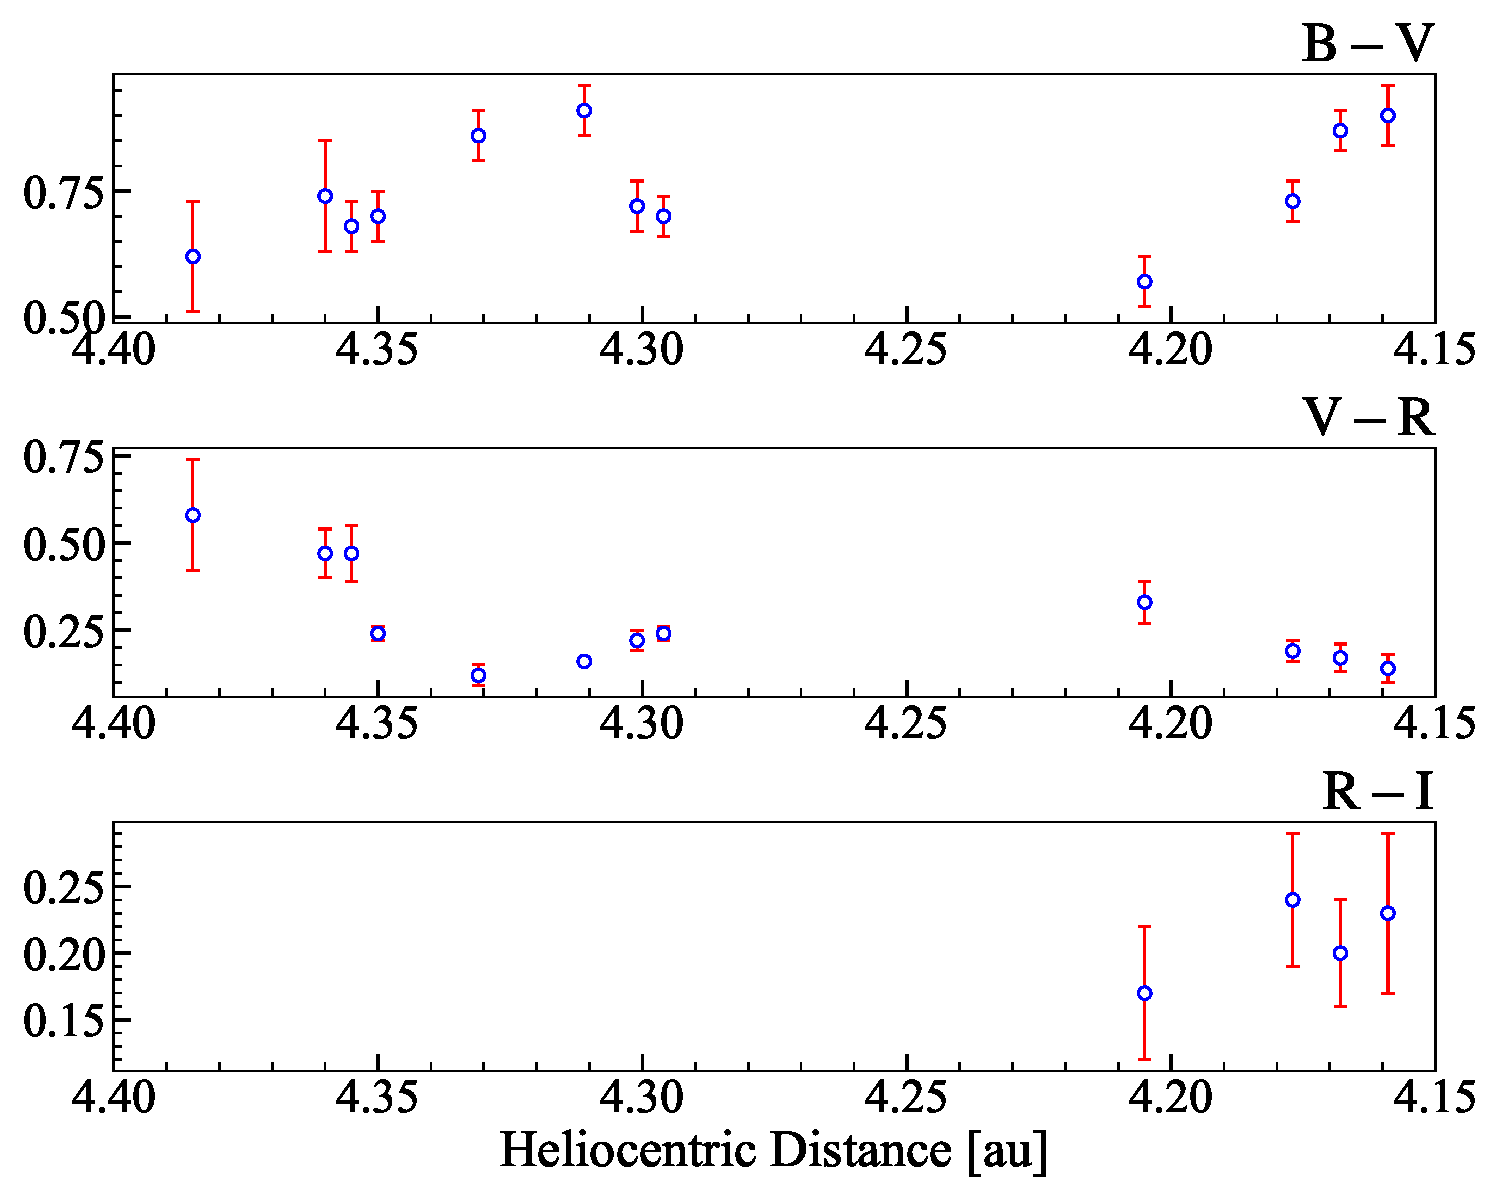
\includegraphics[width=\linewidth]{color-r.pdf} 
    \caption{Color indices vs.\ heliocentric distance for C/2019 L3}\label{fig:color-r}
\end{figure}

Moreover, in order to indicate how the scattered color of the dusty coma varies with wavelengths, the reddening $\mathcal{R}$ (or normalized color) \citep{jewitt_cometary_1986, lara_behaviour_2003, mazzotta_epifani_dust_2011, shi_ccd_2015} is calculated in units of [\si{\percent/\kilo\angstrom}], with the formula given as equation (\ref{eq:red}): 
\begin{equation}
\mathcal{R} = \frac{2}{Af\rho_1 + Af\rho_2} \frac{Af\rho_2 - Af\rho_1}{\lambda_2 - \lambda_1}, 
\label{eq:red}
\end{equation}
where $\lambda_1$ and $\lambda_2$ are the central wavelengths of the filters in units of [\unit{\nm}] (respectively the centers of B and R filters, {\SI{440}{\nm}} and {\SI{658}{\nm}}). With this parameter it is convenient to indicate the percentage of change in the strength of the continuum per {\SI{1000}{\angstrom}}. The results of dust reddening are summarised in Table~\ref{tab:reddening}. In order to avoid the possible effects from background residuals, it is calculated with aperture of {\SI{2e4}{\km}}. 

For comet C/2019 L3, the reddening undergoes significant variations over time, from positive value {\SI{13.75 +- 1.07}{\percent/\kilo\angstrom}} on \DTMdate{2021-3-28} to negative value {\SI{-15.69 +- 0.37}{\percent/\kilo\angstrom}} on \DTMdate{2021-4-12}. We plot the reddening as a function of date in Fig.~\ref{fig:reddening}, and the averaged value {\SI{0.94 +- 0.23}{\percent/\kilo\angstrom}} is marked as a horizontal blue dotted line. For comet C/2020 P3, only on \DTMdate{2021-5-12} is its observational data sufficient for the calcltaion of reddening with a result of {\SI{-6.65 +- 0.01}{\percent/\kilo\angstrom}}. 

The reddening of C/2019 L3 on each observation date is shown in Fig.~\ref{fig:reddening}, with the blue dotted line indicating the mean value. The plot reveals that over the observation course of nearly two months, C/2019 L3 exhibited multiple transitions from a reddish to a bluish color, possibly due to variations in the composition of the coma \citep{ivanova_colour_2017}. 

\begin{table}
    \centering
    \caption{Reddening of comet C/2019 L3 and C/2020 P3 with $\rho = $ \SI{2e4}{\km} }\label{tab:reddening}
    \begin{threeparttable}
        \resizebox{\linewidth}{!}{
        \begin{tabular}{cccc}
            \toprule
            Observation Time & B-band $Af\rho$ & R-band $Af\rho$ & reddening [\si{\%/\kilo\angstrom}]\\
            \midrule
            \multicolumn{4}{l}{\textbf{C/2019 L3}} \\
            2021-03-28.729 & \num{9472 +- 753} & \num{12811 +- 1764} & \num{13.75 +- 1.07}\\
            2021-04-02.739 & \num{8763 +- 806} & \num{10719 +- 617} & \num{9.21 +- 0.50}\\
            2021-04-03.719 & \num{9886 +- 274} & \num{9538 +- 156} & \num{-1.65 +- 0.03}\\
            2021-04-04.691 & \num{9501 +- 343} & \num{8734 +- 93} & \num{-3.86 +- 0.07}\\
            2021-04-08.691 & \num{9288 +- 402} & \num{10797 +- 725} & \num{6.89 +- 0.27}\\
            2021-04-12.724 & \num{12683 +- 602} & \num{8979 +- 113} & \num{-15.69 +- 0.37}\\
            2021-04-14.702 & \num{8809 +- 382} & \num{8700 +- 110} & \num{-0.57 +- 0.01}\\
            2021-04-15.714 & \num{6077 +- 283} & \num{7173 +- 271} & \num{7.59 +- 0.23}\\
            2021-05-04.736 & \num{7724 +- 264} & \num{8065 +- 130} & \num{1.98 +- 0.04}\\
            2021-05-10.735 & \num{9030 +- 285} & \num{8891 +- 154} & \num{-0.71 +- 0.01}\\
            2021-05-12.724 & \num{9044 +- 336} & \num{7958 +- 326} & \num{-5.86 +- 0.16}\\
            2021-05-14.721 & \num{8428 +- 258} & \num{8475 +- 199} & \num{0.25 +- 0.01}\\
            \multicolumn{4}{l}{\textbf{C/2020 P3}} \\
            2021-05-12.749 & \num{934 +- 74} & \num{799 +- 37} & \num{-6.65 +- 0.01}\\
            \bottomrule
        \end{tabular}
        }
    \end{threeparttable}
\end{table}

\begin{figure}
    \centering
    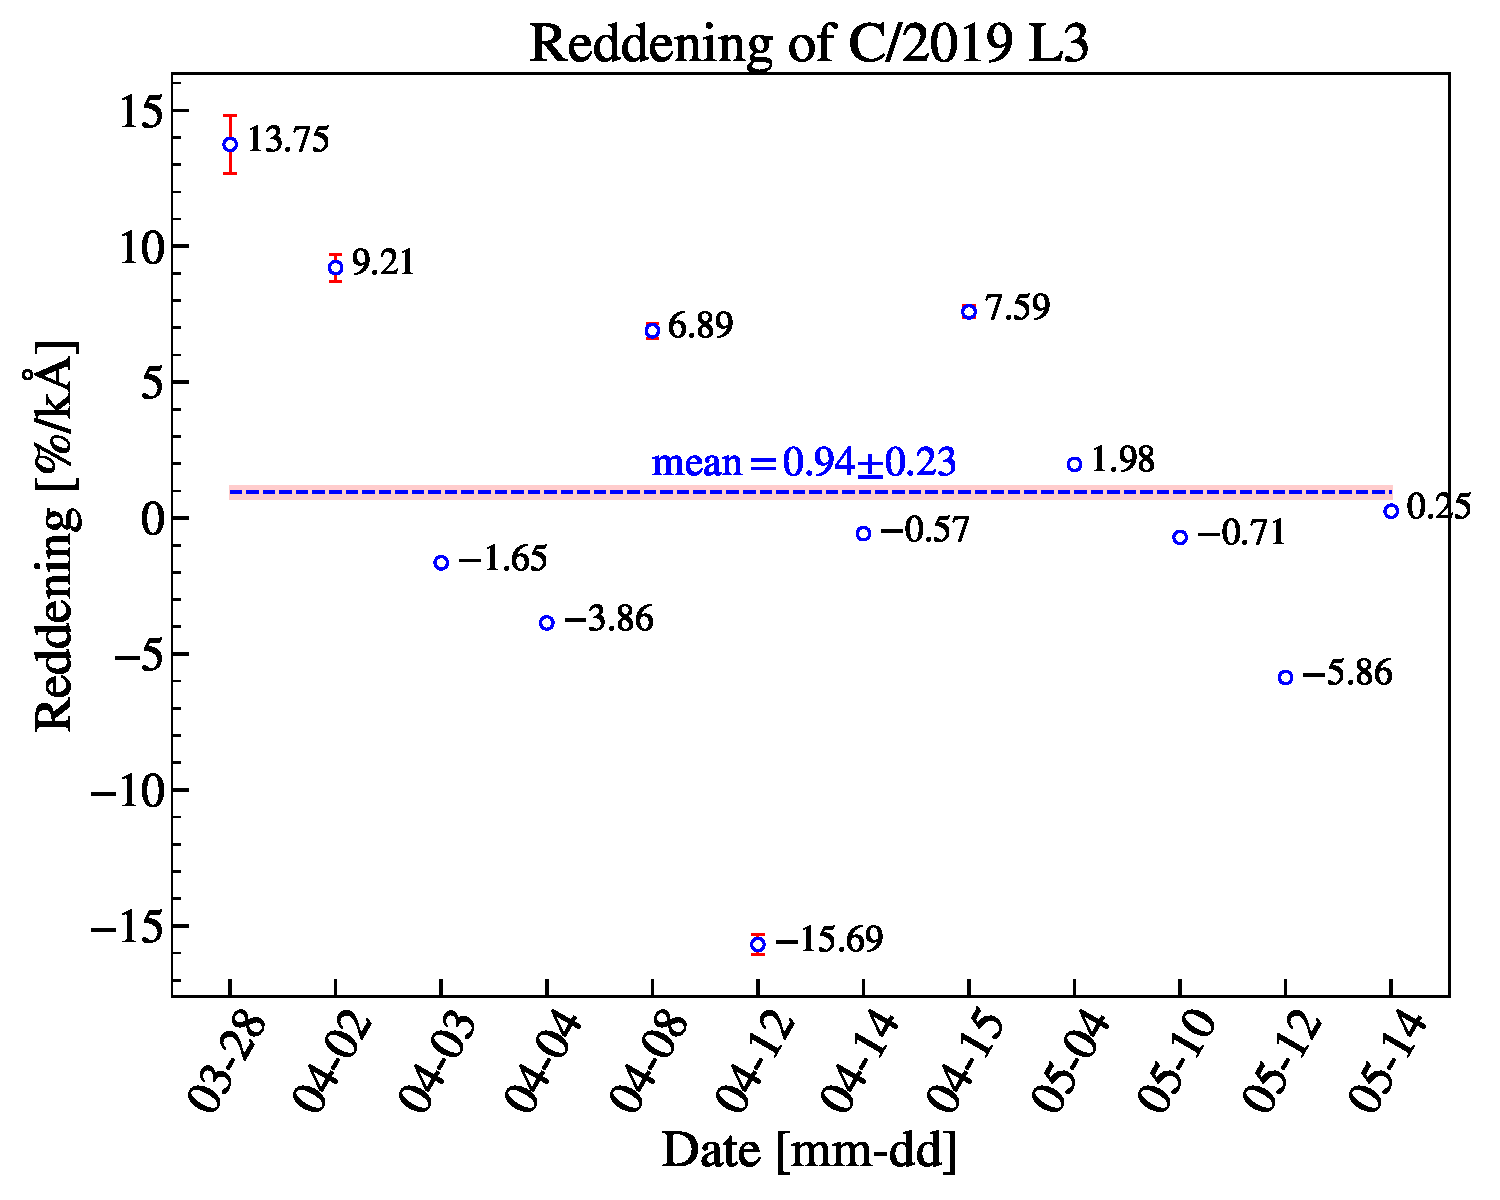
\includegraphics[width=\columnwidth]{reddening.pdf}
    \caption{The reddening of comet C/2019 L3 with date, blue dashed line is the averaged reddening, and the surounding red shadow shows the error. }\label{fig:reddening}
\end{figure}
